\documentclass[11pt]{article}

% Page layout
\usepackage[margin=1in]{geometry}

% Math
\usepackage{amsmath, amsthm, amssymb}
\usepackage{mathtools}

% Tables, figures
\usepackage{booktabs}
\usepackage{graphicx}
\usepackage{multirow}

% Enumerate customisation (leftmargin=* etc.)
\usepackage{enumitem}

% Typography
\usepackage{microtype}
\usepackage{lmodern}
\usepackage[T1]{fontenc}
\usepackage[utf8]{inputenc}

% Hyperlinks
\usepackage[hidelinks]{hyperref}
\usepackage{url}
\usepackage{xurl}  % allow long URLs to break across lines

% References
\usepackage{natbib}
\bibliographystyle{plainnat}

% Theorem environments
\newtheorem{theorem}{Theorem}
% CIT and SIT are observations about the support of the loss, not deep
% results. Naming them as such is deliberate -- see the note after CIT.
\newtheorem{observation}{Observation}
\newtheorem{definition}{Definition}
\newtheorem{hypothesis}{Hypothesis}
\newtheorem{proposition}{Proposition}

% Preprint-specific packages
\usepackage{xcolor}
\usepackage{tikz}
\usepackage{titlesec}

% Colour system for the preprint frontmatter
\definecolor{AugustineNavy}{HTML}{1F3A5F}
\definecolor{AugustineCoral}{HTML}{A50F15}
\definecolor{AugustineGrey}{HTML}{4A4A4A}
\definecolor{LinkBlue}{HTML}{2A5CAA}

\hypersetup{
  colorlinks=true,
  linkcolor=AugustineNavy,
  citecolor=AugustineNavy,
  urlcolor=LinkBlue,
  pdftitle={Chronoception Must Be Installed: The Augustine Problem in LLM Agents},
  pdfauthor={Aojie Yuan},
  pdfsubject={LLM chronoception; position paper}
}

% Project notation
% notation.tex — Chronoception project LaTeX macros
% Source of truth: FRAMING.md §11
% Include in any paper draft with: \input{notation.tex}

% ---- The Three Times ----
\newcommand{\twall}{\tau_{\mathrm{wall}}}
\newcommand{\tstep}{\tau_{\mathrm{step}}}
\newcommand{\tself}{\tau_{\mathrm{self}}}
\newcommand{\tuser}{\tau_{\mathrm{user}}}
\newcommand{\ttoken}{\tau_{\mathrm{token}}}
\newcommand{\treason}{\tau_{\mathrm{reason}}}
\newcommand{\tmin}{\tau_{\min}}

% Realized wall-clock duration under budget B
\newcommand{\twallstar}{\twall^{*}}

% ---- Agent, environment, budget ----
\newcommand{\agent}{A}
\newcommand{\policy}{\pi_{\agent}}
\newcommand{\env}{E}
\newcommand{\tasks}{\mathcal{T}}
\newcommand{\budgets}{\mathcal{B}}
\newcommand{\budget}{B}
\newcommand{\trajectory}{\tau}

% ---- The Three Laws — metrics ----
% L1 Agentic Parkinson coefficient
\newcommand{\parkinson}{\alpha}
% L2 Clock-Adherence Ratio
\newcommand{\CAR}{\mathrm{CAR}}
% L3 Confabulation ratio
\newcommand{\confab}{\rho}

% ---- Central scalar ----
% Chronoceptive Calibration Error
\newcommand{\cce}{\varepsilon}

% ---- Long-horizon success rate ----
\newcommand{\Lsucc}{L}

% ---- Parser for self-narrated duration ----
\newcommand{\selfparser}{\Pi}

% ---- Project-level abbreviations ----
\newcommand{\augustine}{the Augustine Problem}
\newcommand{\Augustine}{The Augustine Problem}
\newcommand{\chrono}{chronoception}
\newcommand{\Chrono}{Chronoception}
\newcommand{\threeTimes}{the Three Times}
\newcommand{\ThreeTimes}{The Three Times}
\newcommand{\CUH}{Chronoception Upstream Hypothesis (CUH)}

% ---- Named laws ----
\newcommand{\LawOne}{Agentic Parkinson's Law (L1)}
\newcommand{\LawTwo}{Step-Clock Conflation (L2)}
\newcommand{\LawThree}{Temporal Confabulation (L3)}

% ---- Project artifacts ----
\newcommand{\ChronoBench}{\textsc{ChronoBench}}
\newcommand{\ChronoStack}{\textsc{ChronoStack}}


% ------- Preprint frontmatter -------
\title{\vspace{-1cm}
  \begin{flushleft}
  \color{AugustineNavy}\rmfamily\bfseries\Huge
  Chronoception Must Be Installed\\[4pt]
  \normalsize\color{AugustineGrey}\rmfamily\itshape
  The Augustine Problem: why LLM agents cannot learn wall-clock time from token-only training.
  \end{flushleft}
}

\author{
  \textbf{Aojie (Justin) Yuan}\\
  University of Southern California\\
  \texttt{aojieyua@usc.edu}
}

\date{\normalsize
  \textbf{Preprint v1.0} \textbullet\ \today\\[6pt]
  \small\color{AugustineGrey}
  \begin{tabular}{@{}rl@{}}
  Code + data + Docker: & \href{https://github.com/Justin0504/Chronoception-agent-temporal-cognition}{\texttt{github.com/Justin0504/Chronoception-agent-temporal-cognition}} \\[1pt]
  Pre-registration:     & \href{https://osf.io/}{\texttt{OSF (locked)}}\ \ \textbullet\ \ \textbf{Correspondence:}\ \texttt{aojieyua@usc.edu} \\
  \end{tabular}
}

\begin{document}
\maketitle
\thispagestyle{empty}

% Framework spine banner
\vspace{-0.4cm}
\begin{center}
\fcolorbox{AugustineNavy!30}{AugustineNavy!5}{
\begin{minipage}{0.95\textwidth}
\small\centering\rmfamily
\textbf{\color{AugustineNavy}The framework's spine.}\ \
Two structural observations \textbf{(CIT, SIT)}, one theorem derived from them \textbf{(Reverse-Scaling)}, three empirical laws \textbf{(L1 / L2 / L3)}, and three papers
\textbf{(Paper 1: this paper; Paper 2: ChronoStack; Paper 3: Agentic Frontier)}.
Layered evidence: (a) \textsc{ChronoBench} \textbf{[14 agents / 7 vendors / $\sim$5{,}900 traj]},
(b) Injection Atlas \textbf{[11 harnesses]}, (c) toy positive control \textbf{[LoRA SFT crosses $\ccestar$]}, (d) HCAST horizon evidence \textbf{[14{,}709 runs]}.
\end{minipage}
}
\end{center}
\vspace{0.15cm}

\begin{abstract}
LLM agents are trained on tokens and deployed in wall-clock time. We argue they cannot close that gap from training alone. Under any loss that is a functional of token sequences --- from next-token prediction through RLHF to reasoning supervision --- the gradient is invariant to how long the episode took, so no amount of scale, context, or reasoning compute installs a representation of elapsed time. \emph{Chronoception must be installed from outside the loss.}

We name the failure the \emph{Augustine Problem}, decompose it along the three times an agent must keep aligned ($\twall$, $\tstep$, $\tself$), and measure it on \textsc{ChronoBench}: 9 sub-capabilities $\times$ 14 agents from 7 vendors, ${\sim}5{,}900$ trajectories. Every agent leaves $\geq 89\%$ of a stated wall-clock budget unspent, and a $60\times$ increase in that budget buys $1.4\times$ more work --- Parkinson's law holds, at a tenth of the strength it requires. Injecting the current date repairs what agents \emph{say}, lifting date accuracy to $\geq 96\%$ panel-wide, and moves what they \emph{do} by $|\Delta\CAR| \leq 0.01$. Three closed labs have independently reached the same workaround, routing the wall-clock into the token stream for consumer products (3/3 inject the date) but not for developer tools (0/3): the harness perceives time on the model's behalf.

Reasoning makes the gap worse rather than better. We show $\mathbb{E}[|\confab| \mid K]$ is monotone non-decreasing in reasoning budget $K$ and confirm it four ways, including a sign flip reproduced on an independent vendor's training pipeline; nominal $90\%$ intervals on self-reported duration achieve $0$--$77\%$ coverage. The consequence is a deployment bound, $T_{\max} \propto 1/\cce$, supported on $14{,}709$ METR HCAST runs (one-sided $p = 0.040$): autonomous-agent horizons are limited by chronoception, not by intelligence.

The field now treats task duration as the variable governing agent reliability, and as the axis along which process-level signals and cost attribution are defined. Each of those programmes presupposes an instrument the policy does not have, and scaling out does not supply it: an orchestrator apportions deadlines its workers cannot perceive.

The gap is structural but not permanent. A LoRA fine-tune on wall-clock-supported targets crosses our calibration threshold after ${\sim}60$\,s of training --- the constructive converse of the impossibility argument, and the shape of what a fix would have to look like. Code, trajectories, and a locked pre-registration are released.
\end{abstract}

\vspace{0.15cm}
\begin{center}
\begin{minipage}{0.94\textwidth}
\small\rmfamily
\textbf{\color{AugustineNavy}How to read this paper.}\ \
The \textbf{position} (\S\ref{sec:intro}) states the claim. The \textbf{ontology} (\S\ref{sec:three-times}) and \textbf{impossibility theorem} (\S\ref{sec:augustine-problem}) formalise it. \textbf{\S\ref{sec:l2}--\ref{sec:injection-tell}} present the layered empirical evidence, one axis at a time. \textbf{\S\ref{sec:epsilon}} aggregates; \textbf{\S\ref{sec:agentic-timeline}} draws the deployment bound; \textbf{\S\ref{sec:future-work}} generalises time to space. \textbf{Readers short on time} may skip to Figure~\ref{fig:reverse-scaling} (the four confirmations of Reverse-Scaling) and Figure~\ref{fig:epsilon-panel} (the 14-agent $\cce$ leaderboard); each carries the paper's central empirical claim in one panel.
\end{minipage}
\end{center}

\vspace{0.2cm}
\hrule
\vspace{0.15cm}
{\small\tableofcontents}
\vspace{0.15cm}
\hrule
\vspace{0.25cm}

% Section 1 — Introduction (compressed for best-paper density)

\section{Introduction}
\label{sec:intro}

A frontier reasoning model, asked how long the next task will take, predicts ``\textit{15 seconds}.'' It thinks for ninety. It answers in two. Pressed for a $90\%$ confidence interval on the duration, the interval contains the truth $0\%$ of the time. None of these failures is a bug or a misread prompt. They are joint, panel-wide, and structurally predictable, present across all 14 agents in our panel.

\paragraph{The Augustine Problem.}
Every training loss in current practice --- next-token cross-entropy, SFT, RLHF, RL with verifiable rewards, reasoning supervision --- is a functional of token sequences. None contains wall-clock time in its support. The models are deployed as agents in continuous physical time. We call the resulting representational gap \emph{the Augustine Problem}, after Augustine's confession that he knew what time was until asked to explain it.\footnote{We use \emph{chronoception} in the cognitive-science sense \citep{wittmann2009chronoception,eagleman2008time}: perception of one's own work duration. Distinct from \citet{goel2025chronocept}'s use for RAG fact validity.} The gap is structural: we prove (Observation~\ref{thm:cit}) that under any token-only loss the policy gradient carries no signal aligning the wall-clock with any internal representation. \emph{Chronoception cannot be acquired from token-only training. It must be installed.}

\paragraph{Position.}
This paper makes that claim precise, measures the failure across the current frontier, audits the industry workaround, and specifies what closing the gap requires. The framework's spine is three theorems (CIT, Reverse-Scaling, SIT), three empirical laws (L1--L3), and three papers (this one, \textsc{ChronoStack}, the Agentic Frontier). The three Times $(\twall, \tstep, \tself)$ of \S\ref{sec:three-times}, illustrated in Fig.~\ref{fig:three-times}, are the framework's fundamental objects.

\paragraph{Layered evidence.}
We support the position with four independent evidence layers: \textbf{(a)} \textsc{ChronoBench}, a 9-capability diagnostic across 14 agents from 7 vendors ($\sim$5{,}900 trajectories), \textbf{(b)} the Injection Atlas, an audit of 11 closed-lab harnesses via leaked system prompts, \textbf{(c)} a toy positive control demonstrating CIT's constructive converse via wall-clock-supported LoRA SFT (Qwen2.5-1.5B crosses $\ccestar$ on T3.1 after $\sim$1\,min of training), \textbf{(d)} horizon-scaling correlational evidence on 14{,}709 public METR HCAST runs.

\paragraph{Contributions.}
\begin{itemize}[leftmargin=1.4em, itemsep=1pt]
\item \textbf{The Augustine Problem} as a named structural diagnosis with a measurable identity $\twall \approx \tstep\!\cdot\!\langle\Delta t\rangle \approx \tself$ (\S\ref{sec:three-times}).
\item \textbf{Two theorems.} CIT (no token-only loss installs chronoception) and Reverse-Scaling ($\mathbb{E}[|\confab|\mid K]$ monotone non-decreasing in reasoning budget $K$); the latter confirmed intra-model, cross-model, within-model, and cross-vendor (\S\ref{ssec:reverse-scaling}).
\item \textbf{ChronoBench and the panel.} 9 sub-capabilities $\times$ 14 agents $\times$ 2 settings, $\sim$5{,}900 trajectories; the Sonnet 4.6 $+$ thinking variant carries the first full $9\!\times\!2\!\times\!30$ panel coverage of any reasoning model (\S\ref{sec:chronobench}).
\item \textbf{The Injection Tell and toy positive control.} $3/3$ consumer web-chat products inject the date, $0/3$ developer tools do (\S\ref{sec:injection-tell}); LoRA SFT with wall-clock-supported targets crosses $\ccestar$ (\S\ref{ssec:a1-positive-control}).
\item \textbf{Deployment bound and spatial mirror.} Agentic Timeline $T_{\max} \propto 1/\cce$ (\S\ref{sec:agentic-timeline}) with HCAST support; generalisation to SIT and the Agentic Frontier $T_{\max}\!\cdot\!S_{\max} \leq C/\ccestST$ (\S\ref{sec:future-work}), the bridge to Papers 2 and 3.
\end{itemize}
Docker container, OSF pre-registration, all trajectories, and the Operational Chronoception Audit Checklist (App.~\ref{app:audit-checklist}) are released.


% Section 2 --- The Three Times (compressed)

\section{The Three Times of an Agent}
\label{sec:three-times}

The introduction gave the failure a name. To make ``failure'' precise we decompose any agent trajectory into three ontologically distinct projections of time (Fig.~\ref{fig:three-times}).

\begin{figure}[h]
\centering
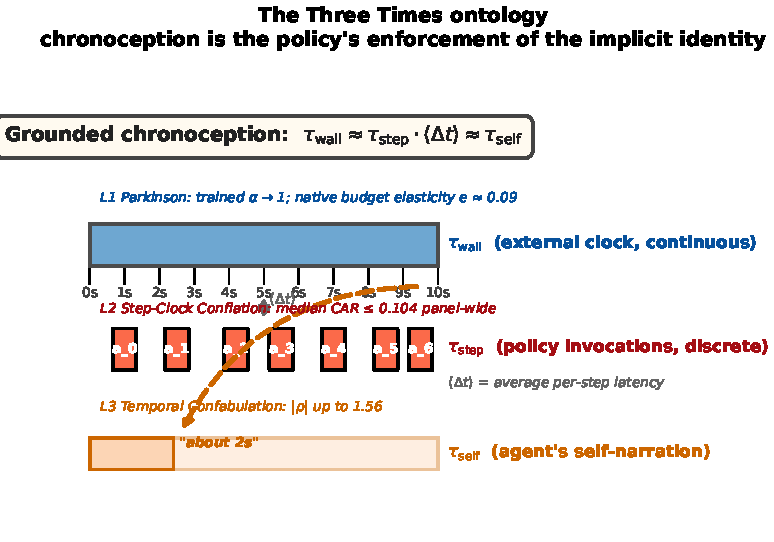
\includegraphics[width=\linewidth]{figures/three_times.pdf}
\caption{The Three Times. $\twall$ (external, continuous), $\tstep$ (discrete policy invocations $a_0, a_1, \ldots$), $\tself$ (agent's narrative of its own duration). A grounded policy enforces $\twall \approx \tstep\!\cdot\!\langle\Delta t\rangle \approx \tself$; the Augustine Problem is failure of this identity. Each axis carries an empirical law (L1--L3).}
\label{fig:three-times}
\end{figure}

\begin{definition}[Three Times]
\label{def:three-times}
For a trajectory $\trajectory = (s_0, a_0, \ldots, s_n)$:
$\twall(\trajectory) := t(s_n) - t(s_0)$ (external timestamp difference);
$\tstep(\trajectory) := n$ (policy invocations);
$\tself(\trajectory) := \selfparser(s_n^{\text{output}})$ (agent-reported duration; parser in App.~\ref{app:annotation-protocol}).
\end{definition}

Grounded chronoception requires
$\twall \approx \tstep \cdot \langle\Delta t\rangle \approx \tself$,
where $\langle\Delta t\rangle$ is the mean per-step wall-clock cost. First approximation is L2; second is L3. The Augustine Problem is joint drift.

\paragraph{Why three, not two or four?} The three are minimal and irreducible. \emph{$\twall \neq \tstep$}: a 10-step trajectory takes $5$\,s on Haiku and $200$\,s on a thinking model. \emph{$\twall \neq \tself$}: agents mis-report by up to $34\times$ (\S\ref{sec:l3}). \emph{$\tstep \neq \tself$}: an agent can produce 6 steps and report ``10 seconds'' with no grounded mapping. Fewer times collapse the training-loss / deployment / narrative arguments; more (e.g., tool-read wall-clock) subsume into $\twall$ once the tool resolves.

With the vocabulary fixed, we can state the Augustine Problem precisely.


% Section 3 — Augustine Problem + CIT (compressed)

\section{The Augustine Problem and Its Impossibility}
\label{sec:augustine-problem}

\begin{definition}[Augustine Problem]
\label{def:augustine-problem}
Agent $A$ exhibits the Augustine Problem on task family $\tasks$ if
$\mathbb{E}_{\trajectory \sim \pi_A}\!\left[|\twall - \tstep\langle\Delta t\rangle| + |\twall - \tself|\right] > \cce_0$
for some tolerance $\cce_0$. The three projections drift independently across the trajectory distribution.
\end{definition}

The question is not whether agents exhibit it (they do, \S\ref{sec:l2}--\ref{sec:l3}) but whether any conceivable foundation-model training procedure could in principle close it. We argue: not by scale, not by reasoning-compute expansion, not by any post-training intervention on token sequences alone.

\paragraph{Assumption (token-only loss support).}
\label{ass:token-only}
A training procedure is in the \emph{token-only regime} if
$\loss(\theta) = \mathbb{E}_{x \sim \mathcal{D}}[\ell(f_\theta(x_{<i}), x_i)]$
satisfies (i) $\mathcal{D}$ is a distribution over finite token sequences with no field carrying wall-clock duration, and (ii) $\ell$ is a function of the output token distribution alone. Next-token cross-entropy, SFT, RLHF, RL with verifiable rewards, and reasoning supervision all satisfy this.

\begin{observation}[Chronoception Impossibility, CIT]
\label{thm:cit}
Let $\loss$ be a token-only loss. For any strictly increasing $\phi: \mathbb{R}_{>0} \to \mathbb{R}_{>0}$, $\loss(\theta)$ is invariant under $\twall \mapsto \phi(\twall)$. Equivalently, $\nabla_\theta \loss$ carries zero gradient signal aligning $\twall$ with any internal representation.
\end{observation}

\begin{proof}[Sketch]
$\nabla_\theta\loss = \mathbb{E}[\partial\ell/\partial f_\theta \cdot \nabla_\theta f_\theta]$. Neither factor depends on the wall-clock time at which the sample was generated: tokens carry no timestamps, $\ell$ is a function of the output distribution alone. The gradient is therefore invariant to any reparametrisation of $\twall$. A policy from this gradient cannot distinguish one wall-clock duration from another.
\end{proof}

\paragraph{On calling this an observation.} The argument above is two lines
long and follows from the definition of the loss. We do not present it as a
deep result and have named it accordingly. Its value is not that it is hard to
prove but that it is rarely stated and its consequences are almost never drawn:
the field routinely expects longer context, more parameters or more reasoning
tokens to improve an agent's handling of its own runtime, and Observation~1
says none of them can, because none of them changes what the loss can see. A
claim can be immediate and still be load-bearing. What has to be earned is not
the observation but everything after it --- that the gap it predicts is
actually there, at what size, in which direction under reasoning-token
expansion, and what it costs at deployment. That is what the rest of this paper
measures.

\paragraph{Scope.} CIT does not claim there is \emph{no} internal representation of time; it claims any such representation is not produced \emph{by the loss}. Explicitly out of scope: harness-installed chronoception (\S\ref{sec:injection-tell}, a CIT workaround, not refutation), tool-output-installed chronoception (calling \texttt{date}), and future losses with $\twall$ as an explicit argument (\textsc{ChronoStack}). CIT precludes only the inference --- widely held, rarely defended --- that additional scale, longer reasoning, or larger context will close the gap.

\paragraph{Empirical predictions.} \textbf{(P-CIT-1)} $\CAR$ stays bounded away from 1 regardless of capability (\S\ref{sec:l2}). \textbf{(P-CIT-2)} Prompt-level wall-clock information cannot move action-axis behaviour (Prop.~\ref{prop:injection-not-action}). \textbf{(P-CIT-3)} Calibration tooling cannot close self-duration calibration (\S\ref{ssec:calibration}). All three are confirmed by the panel.

\paragraph{Augustine Threshold.} We adopt $\ccestar = 0.20$ as an operational reporting threshold, and we are explicit about its status. It is \emph{not} derived from a measured human baseline. Human duration perception is itself imperfect and strongly scale-dependent \citep{wittmann2009chronoception,eagleman2008time}, which is the qualitative motivation for setting the bar below perfection rather than at it --- but that literature reports \emph{discrimination} thresholds (Weber fractions on whether two intervals differ), not the \emph{retrospective estimation} error that $\confab$ measures, and the two are not interconvertible without an argument we cannot currently supply. We therefore fix $\ccestar = 0.20$ by stipulation: the round figure roughly one order of magnitude below a $2\times$ misestimate ($|\confab| = \log_{10} 2 \approx 0.30$). It was chosen before the panel was run and held fixed afterwards.

We flag this because the threshold is the one place a reader might expect a derivation and not find one. Nothing in the argument depends on the constant. The closest agent sits at $\cce = 0.536$, and $\mathrm{score}_{T_2} \geq 0.92$ on every agent in the panel puts a floor of $\cce \geq 0.46$ under the whole panel irrespective of the narrative axis, so every qualitative conclusion here survives any choice of threshold in $[0.1, 0.45]$. A task-matched human panel would let $\ccestar$ be earned rather than stipulated, and is the highest-priority follow-up (\S\ref{sec:limitations}). No panel agent crosses it (\S\ref{sec:epsilon}).

CIT says the gap is unavoidable. To measure ``unavoidable'' we need the instrument next.


% Section 4 --- ChronoBench (v4)

\section{ChronoBench: A Diagnostic Instrument for the Three Axes}
\label{sec:chronobench}

To decide whether CIT's three predictions (\S\ref{sec:augustine-problem}) hold on real agents, we need instruments that measure each of the Three Times \emph{independently}. Aggregate benchmarks obscure what we want to see: a failure on a hard SWE-Bench task may be a chronoception failure, a reasoning failure, or a tool-use failure, and no aggregate metric will tell them apart. \textsc{ChronoBench}'s design philosophy is therefore single-axis isolation: every instance loads on exactly one of $\twall$, $\tstep$, or $\tself$, so a failure is unambiguously attributable to the axis under test. We summarise the 9 sub-capabilities here; the full prompt set, panel composition, parser specification, and open-source serving recipe appear in Appendix~\ref{app:annotation-protocol}.

\begin{table}[h]
\centering
\caption{The 9 sub-capabilities of \textsc{ChronoBench}, three per axis. Each row isolates a single chronoceptive failure mode for separate measurement and pairs it with the diagnostic question a deployment auditor should ask.}
\label{tab:capabilities}
\small
\begin{tabular}{@{}llp{4.6cm}p{4.2cm}@{}}
\toprule
Axis & Sub-capability & Tests & Auditor question \\
\midrule
\multirow{3}{*}{$\twall$}
 & T1.1 Clock awareness       & Today's date / current time      & ``\emph{Does it know when it is?}'' \\
 & T1.2 Elapsed-time tracking & Time since conversation start    & ``\emph{Does it track elapsed time?}'' \\
 & T1.3 Deadline tradeoff     & Strategy under wall-clock deadline & ``\emph{Does it re-plan under pressure?}'' \\
\midrule
\multirow{3}{*}{$\tstep$}
 & T2.1 Step-budget honouring & Produce exactly $N$ steps        & ``\emph{Can it count its steps?}'' \\
 & T2.2 Step-to-wall map      & Compute $N\!\times\!\Delta t = \tau$ & ``\emph{Can it convert step to wall-time?}'' \\
 & T2.3 Wall-budget execution & Honour a wall-clock budget (L2)  & ``\emph{Does the budget change behaviour?}'' \\
\midrule
\multirow{3}{*}{$\tself$}
 & T3.1 Retrospective $\confab$ & Duration reported after task   & ``\emph{How long did it just take?}'' \\
 & T3.2 Prospective $\confab$   & Duration predicted before task & ``\emph{How long will this take?}'' \\
 & T3.3 Calibration             & 90\% CI over self-duration     & ``\emph{How confident in its duration?}'' \\
\bottomrule
\end{tabular}
\end{table}

\paragraph{Settings.}
Every instance runs under two settings. Setting A uses a vanilla system prompt (``\textit{You are a helpful assistant.}'') and supplies no harness-side wall-clock signal. Setting B prepends ``\textit{Current date and time: \{ISO\}}'' to the system prompt, emulating the consumer web-chat behaviour documented in \S\ref{sec:injection-tell}. The contrast between A and B isolates injected information from policy-internal representation.

\paragraph{Panel.}
Fourteen agent configurations from seven providers: \textbf{OpenAI's} gpt-4o-mini, gpt-4o, gpt-5.1, o3, and o4-mini (three \texttt{reasoning\_effort} levels); \textbf{Anthropic's} Claude Haiku 4.5 and Claude Sonnet 4.6 (with and without extended thinking, 8k-token budget); \textbf{open-source} Qwen2.5-7B and DeepSeek-R1-Distill-Qwen-14B (three \texttt{max\_completion\_tokens} budgets), both self-hosted via vLLM on a single 8$\times$RTX 6000 Ada cluster; and a \textbf{cross-vendor Chinese-lab expansion} via Vultr Inference: Z.AI's \textbf{GLM-5.2-FP8}, MiniMax's \textbf{MiniMax-M2.7}, Moonshot's \textbf{Kimi-K2.6}, and Alibaba's \textbf{Qwen3.6-27B}. The o4-mini reasoning-effort sweep and the Sonnet 4.6 thinking variant supply the empirical basis for the Reverse-Scaling Theorem (\S\ref{ssec:reverse-scaling}); the Chinese-lab expansion tests whether the framework's predictions hold across a distinct training pipeline and vendor ecosystem. We collect 30 trajectories per (model, capability, setting) cell, for a total of roughly $5{,}900$ trajectories --- with the Sonnet 4.6 $+$ extended-thinking variant carrying the first full $9\!\times\!2\!\times\!30$ panel coverage of any reasoning model.

\paragraph{Implementation and release.}
\textsc{ChronoBench} ships as a \texttt{pip}-installable Python package with a command-line interface and three backend adapters (OpenAI, Anthropic, OpenAI-compatible for vLLM/Ollama). The metric library implements $\parkinson$, $\CAR$, $\confab$, and the aggregate $\cce$. All trajectories, parser outputs, and analysis scripts are released; a Docker container reproduces every figure and table from the committed data in approximately five minutes.

With the instrument fixed, we can test CIT one axis at a time. We begin with the action axis, because that is where CIT's first prediction is sharpest and its consequences most consequential for deployment.


% Section 4b — L1 Agentic Parkinson, measured as a budget elasticity

\section{The Wall Axis: L1 Measured, Not Assumed}
\label{sec:l1}

Of the three laws, L1 is the one we could most easily have left as an
assertion. Parkinson's observation that ``work expands so as to fill the time
available'' \citep{parkinson1955} is the folk theory of what a budgeted agent
does, and an earlier draft of this paper stated its contrapositive --- that
native agents simply do not exhibit it --- on the strength of the $\CAR$
numbers in \S\ref{sec:l2}. That statement was wrong, and the corpus already
contained the data to show it.

\paragraph{Why not T1.3.} T1.3 is the sub-capability nominally assigned to
L1, and it cannot answer the question. Its trajectories carry
\texttt{budget\_kind="none"}, so the stated deadline lives only inside the
prompt string and $\parkinson$ is not computable from them. More seriously,
its ten prompts pair each deadline with a different question, and the pairing
tracks intrinsic task size almost perfectly: the five-second item asks for the
capital of Australia, the 180-second item asks for a short story. Deadline and
task size are confounded, so a longer answer under a longer deadline is
uninformative. No reanalysis repairs this; the design has to be re-run
crossed, which we describe in \S\ref{sec:limitations}.

\paragraph{The design L1 needs is already in T2.3.} The wall-budget
capability holds the task fixed and varies the budget over
$\budget \in \{60, 300, 900, 1800, 3600\}$\,s at $n = 30$ per cell per
setting --- a $60\times$ range on a single factor. We therefore measure L1 as
a \emph{budget elasticity},
\[
  e \;:=\; \frac{\mathrm{d}\,\log_{10} \twallstar}{\mathrm{d}\,\log_{10} \budget},
\]
fit per agent by least squares over all $(\budget, \twallstar)$ pairs with a
$95\%$ bootstrap CI ($4{,}000$ resamples). Parkinson's law in its strong form
is $e = 1$: the work expands to fill whatever it is given. Complete
indifference to the budget is $e = 0$.

\begin{table}[h]
\centering\small
\caption{L1 budget elasticity across the panel. $e = 1$ is Parkinson's law in
full; $e = 0$ is no response to the budget at all. Pooled over both settings,
$n = 60$ per agent.}
\label{tab:l1-elasticity}
\begin{tabular}{lcc|lcc}
\toprule
Agent & $e$ & 95\% CI & Agent & $e$ & 95\% CI \\
\midrule
Claude Haiku 4.5 & $+0.228$ & $[+0.170, +0.284]$ & MiniMax-M2.7   & $+0.089$ & $[+0.028, +0.147]$ \\
GLM-5.2-FP8      & $+0.219$ & $[+0.166, +0.272]$ & gpt-4o-mini    & $+0.082$ & $[-0.141, +0.219]$ \\
gpt-5.1          & $+0.149$ & $[+0.102, +0.202]$ & Sonnet $+$ thinking & $+0.074$ & $[-0.038, +0.185]$ \\
o3               & $+0.127$ & $[+0.062, +0.196]$ & o4-mini        & $+0.072$ & $[+0.028, +0.131]$ \\
gpt-4o           & $+0.103$ & $[+0.068, +0.139]$ & Qwen3.6-27B    & $+0.058$ & $[+0.036, +0.079]$ \\
Kimi-K2.6        & $+0.092$ & $[+0.027, +0.156]$ & Claude Sonnet 4.6 & $+0.052$ & $[+0.021, +0.090]$ \\
                 &          &                    & Qwen2.5-7B     & $-0.020$ & $[-0.099, +0.061]$ \\
\midrule
\multicolumn{6}{l}{\textbf{Panel median $e = 0.089$}; 10 of 13 agents have a CI strictly above zero.} \\
\bottomrule
\end{tabular}
\end{table}

\paragraph{Result: present, and an order of magnitude too weak.}
The panel median is $e = 0.089$, and ten of thirteen agents across seven
vendors have a bootstrap CI strictly above zero (Table~\ref{tab:l1-elasticity}).
A $60\times$ increase in the stated budget therefore buys $1.4\times$ more
wall-clock, where Parkinson's law requires $60\times$. A single exponent
describes each agent's ladder to between $3\%$ and $22\%$ (median ${\sim}12\%$),
so the power-law summary is a reasonable description of the budget response and
not a line drawn through noise.

This is the narrative/action split of \S\ref{sec:l2}--\ref{sec:l3} visible on a
single axis. The agent's response to the budget is \emph{directionally correct}
--- it reads the number and moves the right way --- and it is roughly a tenth of
the strength the instruction calls for. An agent that could not read the budget
at all would give $e = 0$; an agent that could act on what it read would give
$e = 1$. The panel sits an order of magnitude from the second and, for most
agents, reliably away from the first.

\paragraph{What this is not.} Two limits bound the claim, and both point at the
same missing experiment. First, T2.3 is a \emph{single task}: $e$ is measured on
one item, so we cannot say whether the elasticity is a property of the agent or
of that item. Second, the T2.3 prompt explicitly instructs the agent to spend
the budget (``\textit{work on this task for $\budget$ seconds; do not stop
early}''), so $e$ measures compliance with an instruction, not the spontaneous
expansion Parkinson described. That makes $e = 0.089$ an \emph{upper bound} on
spontaneous L1 rather than a measurement of it --- which strengthens the
direction of the finding while weakening its interpretation as Parkinson's law
proper. The crossed design that would fix both, questions $\times$ deadlines
fully crossed with the budget recorded as a field, is specified in
\S\ref{sec:limitations}.

\paragraph{Relation to $\CAR$.} Since $\CAR = \twallstar/\budget$, we have
$\mathrm{d}\log \CAR / \mathrm{d}\log \budget = e - 1$ identically. The steep
decay of $\CAR$ with budget reported in \S\ref{sec:l2} is therefore the same
measurement in different coordinates, not independent corroboration of it, and
we do not present it as such. What the two views jointly establish is that one
exponent near zero governs both: the agent's wall-clock expenditure is nearly
invariant to what it is told it has.


% Section 5 --- L2 Step-Clock Conflation (compressed)

\section{The Action Axis: L2 Step-Clock Conflation}
\label{sec:l2}

CIT-P1 predicts the action axis cannot honour wall-clock budgets. We ask each agent ``\textit{work on this task for $\budget$ seconds; do not stop early},'' vary $\budget \in \{60, 300, 900, 1800, 3600\}$\,s ($n=30$ per budget, both settings), and measure the Clock-Adherence Ratio $\CAR(\budget) := \twallstar/\budget$.

\begin{definition}
A chronoceptively grounded agent satisfies $\CAR \approx 1$; an L2-failing agent satisfies $\CAR \ll 1$ once $\budget \gg \tmin$.
\end{definition}

\paragraph{Result.} No panel agent's median $\CAR$ exceeds $0.104$ and the panel median is $0.014$: every agent leaves at least $89\%$ of the budget it was given unspent, and the non-reasoning core leaves over $95\%$. Wall-clock injection does not move the number (Table~\ref{tab:l2-car}).

\begin{table}[h]
\centering
\small
\caption{Median $\CAR$ across the 13-cell post-B-1 panel. Injection moves the action axis by at most $\pm 0.005$.}
\label{tab:l2-car}
\begin{tabular}{lccc}
\toprule
Model & $\CAR$ (A) & $\CAR$ (B) & $|\Delta \CAR|$ \\
\midrule
\multicolumn{4}{l}{\textit{Non-reasoning core panel}} \\
gpt-4o-mini, gpt-4o, gpt-5.1, Haiku 4.5, Sonnet 4.6, Qwen2.5-7B & $0.004$--$0.050$ & $0.004$--$0.050$ & $\leq 0.008$ \\
\midrule
\multicolumn{4}{l}{\textit{Reasoning models}} \\
o3 & 0.011 & 0.009 & 0.002 \\
o4-mini & 0.008 & 0.007 & 0.001 \\
Sonnet 4.6 $+$ thinking & 0.100 & 0.104 & 0.004 \\
\midrule
\multicolumn{4}{l}{\textit{Chinese-lab expansion}} \\
GLM-5.2, MiniMax-M2.7, Kimi-K2.6, Qwen3.6-27B & $0.011$--$0.024$ & $0.010$--$0.021$ & $\leq 0.003$ \\
\midrule
Panel median & \textbf{0.014} & \textbf{0.014} & 0.001 \\
\bottomrule
\end{tabular}
\end{table}

\paragraph{The $60$\,s tier, where the sign flips.} The medians above pool five budgets, and that pooling hides the one place the failure changes shape. At $\budget = 60$\,s every reasoning model's $\CAR$ is an order of magnitude above its pooled median (o3 $0.225$, o4-mini $0.159$), and Sonnet 4.6 $+$ thinking \emph{overshoots} outright at $\CAR = 2.22$: the extended-thinking policy cannot bring itself to stop inside a minute and blows through the budget by more than a factor of two. This is not a counter-example to L2 but its cleanest illustration. A policy with a representation of $\twall$ would track the budget from either side; these policies miss it from whichever side their default generation length happens to fall on, and the sign of the miss is set by that default rather than by the budget. Under-spend and overshoot are the same failure of the identity $\twall \approx \tstep\langle\Delta t\rangle$, read at two different budget scales.

\paragraph{The narrative-vs-action split.}
Across five non-reasoning generations $|\confab|$ falls $94\%$ (\S\ref{sec:l3}) while median $\CAR$ stays at $0.01$--$0.05$: narrative axis is text-trainable, action axis is not. Injection is an information intervention (rewrites the prompt) but not a representational one (does not learn a $\twall$-to-action mapping). The action axis is unmoved. The empirical signature $|\Delta\CAR| \leq 0.01$ across the 13-cell panel and three separate vendor ecosystems (western labs, Chinese labs, open source) formalises this as:

\begin{proposition}[Injection cannot install action-axis chronoception]
\label{prop:injection-not-action}
Let $A$ be an agent in the token-only regime (Assumption~\ref{ass:token-only}) and $A_B$ the same policy under Setting B. Then $\CAR(A_B) - \CAR(A) = 0$ in expectation to the order of the policy's prompt-token sensitivity. Injection is a narrative-axis intervention; it can rewrite what the agent \emph{says} about time but not what the agent \emph{does} with time.
\end{proposition}

\begin{proof}[Sketch] Injection extends the token prefix by a constant string. By CIT the policy's prefix-to-action-selection map is time-reparametrisation-invariant on the training manifold. Prefix-level information about $\twall$ modifies output-token generation but not the wall-clock realisation of the action sequence. The empirical $|\Delta\CAR| \leq 0.01$ across the panel is direct measurement of the proposition. \end{proof}

L2 is the load-bearing empirical claim: it anchors $\cce$ above $\ccestar$ for every panel agent (\S\ref{sec:epsilon}) and bounds the Agentic Timeline regardless of capability scaling (\S\ref{sec:agentic-timeline}). The next section turns to the narrative axis, where capability scaling helps monotonically --- and Reverse-Scaling structurally undoes the help.


% Section 6 — L3 Temporal Confabulation (compressed for best-paper density)

\section{The Narrative Axis: Closure, Ceiling, and Catastrophe}
\label{sec:l3}

Section~\ref{sec:l2} showed capability scaling does not help the action axis. This section is its counterpoint: on the narrative axis $\confab := \log_{10}(\tself/\twall)$, capability scaling helps monotonically across five frontier non-reasoning generations ($|\confab|$ from $+1.12$ to $+0.07$, a $94\%$ reduction; full table in App.~\ref{app:full-panel-tables}). The closure is real; it is also bounded in three directions, each with its own \S: a theorem that reasoning-token expansion \emph{reverses} the trend (\S\ref{ssec:reverse-scaling}), a calibration catastrophe that persists even where the surface appears closed (\S\ref{ssec:calibration}), and a constructive positive control that shows what training would actually close it (\S\ref{ssec:a1-positive-control}).

\subsection{The Reverse-Scaling Theorem}
\label{ssec:reverse-scaling}

\paragraph{Assumption (budget-honoured reasoning).}
\label{ass:budget-honoured}
A reasoning-budget knob $K$ on a fixed agent is \emph{honoured} if $\mathbb{E}[\twall \mid K]$ is strictly increasing in $K$. The o4-mini \texttt{reasoning\_effort} ladder, Anthropic extended-thinking budget, and Kimi/GLM reasoning modes all satisfy this empirically. Budgets the model declines to spend (E5 on DeepSeek-R1-Distill-14B, App.~\ref{app:l3-detail}) fall outside the assumption and are not counter-examples.

\begin{theorem}[Reverse-Scaling]
\label{thm:reverse-scaling}
For a fixed agent under Assumption~\ref{ass:token-only} (hence Observation~\ref{thm:cit}) with a budget-honoured $K$, $\mathbb{E}[|\confab| \mid K]$ is monotone non-decreasing in $K$.
\end{theorem}

\begin{proof}[Sketch]
Under CIT, $p(\tself)$ is invariant to $\twall$: no gradient signal ties one to the other. The inference-time distribution $p(\tself \mid K) = p(\tself)$ for all $K$. By assumption, $\twall(K)$ is strictly increasing. Therefore $|\log_{10}(\tself/\twall)|$ is monotone non-decreasing in $K$ in expectation. The sign of $\confab$ turns negative once hidden CoT comes to dominate $\twall$, because $p(\tself)$ stays anchored to the surface output; the theorem itself constrains only $|\confab|$.
\end{proof}

\begin{figure}[h]
\centering
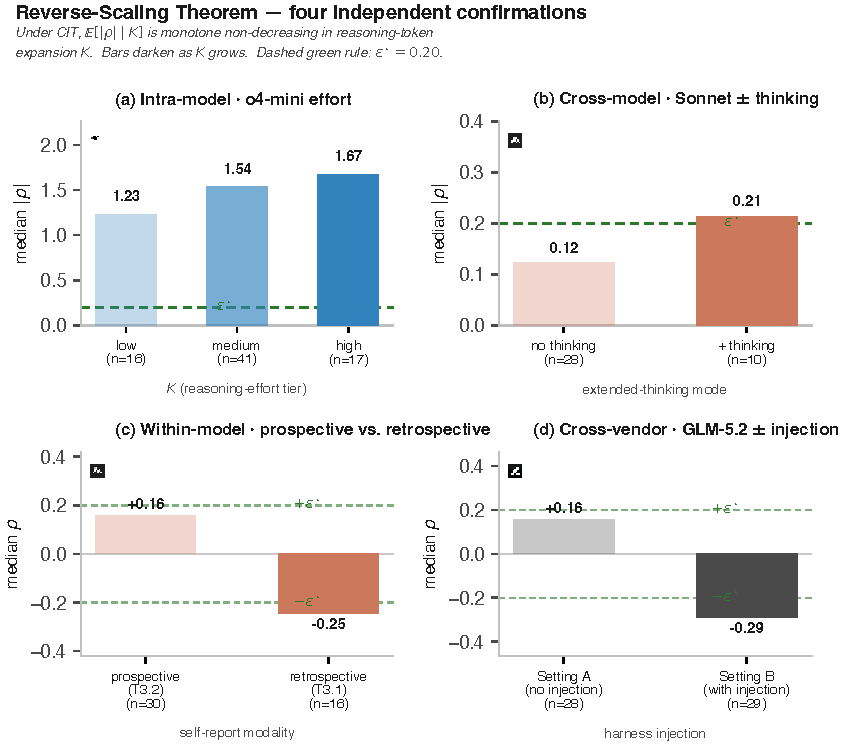
\includegraphics[width=\linewidth]{figures/reverse_scaling.pdf}
\caption{Four independent confirmations of Theorem~\ref{thm:reverse-scaling}. \textbf{(a)} Intra-model: o4-mini \texttt{reasoning\_effort} ladder, $|\confab| = 1.23 \to 1.54 \to 1.67$. \textbf{(b)} Cross-model: Sonnet 4.6 $\pm$ extended thinking, median $|\confab| = 0.12 \to 0.21$ (Setting~A, $n = 28/10$; signed median $+0.07 \to -0.17$), with the sign flip firm under Setting~B ($-0.25$, CI $[-0.34, -0.11]$, $n = 16$). \textbf{(c)} Within-model: Sonnet-thinking prospective ($+0.16$) vs.\ retrospective ($-0.25$) under Setting~B --- sign flip on the same tasks. \textbf{(d)} Cross-vendor: GLM-5.2 (Z.AI, no shared training pipeline with Anthropic), Setting~A $\to$ B: $+0.16 \to -0.29$. Detailed per-cell CIs in App.~\ref{app:full-panel-tables} Tables~\ref{tab:full-panel}--\ref{tab:reasoning-t3}.}
\label{fig:reverse-scaling}
\end{figure}

The four confirmations vary four independent things: reasoning effort within one model, the presence of a thinking mode across two builds of one model, the narration modality within one configuration, and the training pipeline across two vendors that share none of it. All four show the same object --- raising the reasoning budget, or triggering reasoning-mode CoT, grows $|\confab|$. Three of the four also flip its sign toward Hidden-Time under-report, and on Setting~B the three Chinese-lab reasoning models (GLM-5.2, Kimi-K2.6, Qwen3.6-27B) sit collectively at median $\rho \in [-0.97, -0.29]$, which makes the flip a property of the class rather than of Sonnet-thinking.

It is not universal, and we say so: o3 grows $|\confab|$ to $0.45$ --- well above base Sonnet 4.6's $0.12$ on the same tasks --- while continuing to over-report (App.~\ref{app:full-panel-tables}). Theorem~\ref{thm:reverse-scaling} constrains the magnitude, and every cell confirms the magnitude. The sign flip is the mechanism's most visible symptom, not its definition: it appears when the hidden chain-of-thought comes to dominate $\twall$, and o3 is the configuration where it does not.

\subsection{Who Declines to Answer}
\label{ssec:refusal}

The panel tables report an effective $n_\rho$ ``after parser drops''. That
single number turns out to cover four behaviours which mean different things,
and separating them changes how two of our own results should be read.
Classifying all $900$ T3.1 trajectories (App.~\ref{app:l3-detail}): $626$ state
a positive duration and are scored; of the $274$ that are not, $110$ ($40\%$)
are an \emph{explicit refusal} to estimate, $132$ ($48\%$) never mention
duration, $18$ ($7\%$) state a duration of exactly zero, and $14$ ($5\%$) are
positive durations our scorer missed.

\paragraph{Reasoning-mode agents refuse an order of magnitude more often.}
Refusals are not spread evenly. Pooled over settings, reasoning-mode
configurations decline on $21.9\%$ of trajectories ($n = 480$) against $1.2\%$
for non-reasoning ($n = 420$) --- an $18\times$ gap. Sonnet 4.6 $+$ thinking
declines on $57\%$, Kimi-K2.6 on $42\%$, gpt-5.1 on $35\%$, while gpt-4o,
gpt-4o-mini, Haiku 4.5, Qwen2.5-7B and Qwen3.6-27B never once decline. This is
the same object as the cross-lingual refusal asymmetry of
\S\ref{sec:limitations}, seen on the narrative axis instead of the wall axis:
declining to estimate is a surface disposition of post-training, distributed
very unevenly across configurations, and not a representation of the
underlying absence.

\paragraph{Two consequences we report rather than absorb.}
First, $\rho$ for the high-refusal agents is computed on a \emph{selected}
subsample --- the trajectories where the agent chose to commit a number.
Sonnet 4.6 $+$ thinking's $n_\rho = 10$ under Setting~A is not a parsing
failure but a $57\%$ refusal rate, and its contribution to the cross-model
sign flip (Fig.~\ref{fig:reverse-scaling}b) therefore rests on the $43\%$ where
it answered. We cannot bound the direction of that selection from these data;
the intra-model effort ladder and the cross-vendor comparison, whose agents
refuse at $13\%$ and $5\%$, do not carry the same exposure, and the theorem's
magnitude claim is confirmed on all of them.

Second, the $18$ trajectories reporting \emph{exactly zero} seconds are
excluded by the arithmetic rather than by choice: $\rho = \log_{10}(0/\twall)$
is undefined. These are the most extreme under-reports the instrument can
produce, so every $|\confab|$ we report is, by that much, an underestimate. The
bias runs against our own claim, which is the direction we would rather it ran,
but it should be stated.

\subsection{The Calibration Catastrophe}
\label{ssec:calibration}

Asked to wrap self-duration in a $90\%$ confidence interval, every non-reasoning panel agent achieves under-coverage of at least $40$ percentage points (Fig.~\ref{fig:calibration-catastrophe}); GPT-4o reaches $0\%$. Standard post-training calibration tooling (temperature scaling, isotonic regression, RLHF-with-confidence \citep{guo2017calibration,jiang2021calibration,kadavath2022knowing,dontthinktwice2025}) cannot apply, because the calibration signal is not in the loss support (CIT). Pre-registered P11: no CIT-regime agent achieves $> 0.5$ coverage without harness-side duration data.

\begin{figure}[h]
\centering
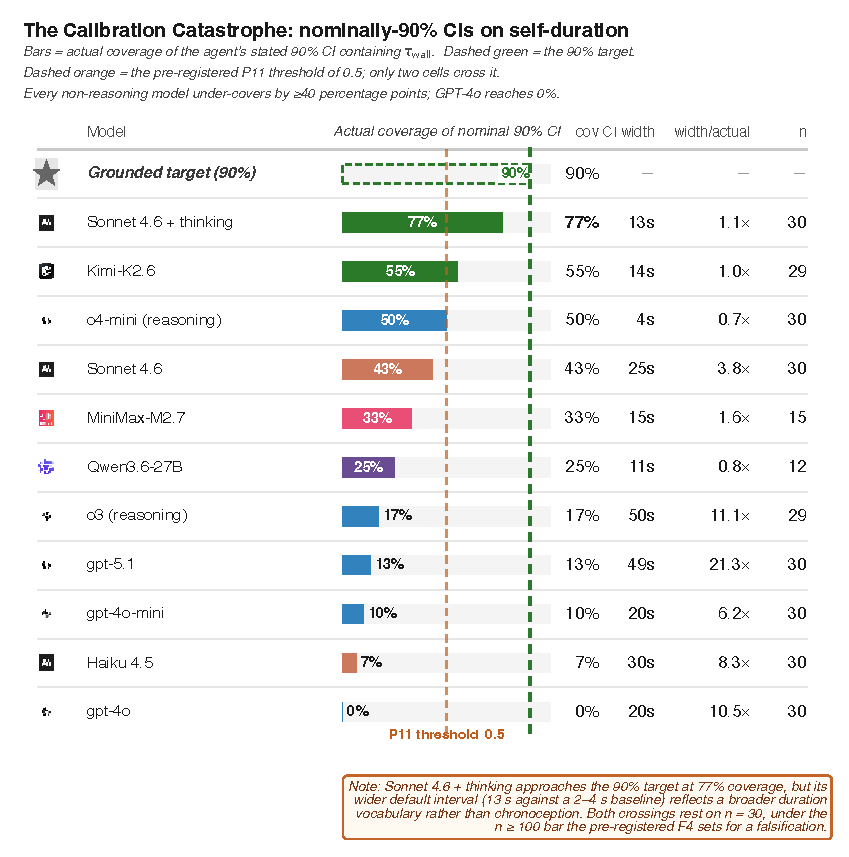
\includegraphics[width=\linewidth]{figures/calibration_catastrophe.pdf}
\caption{Actual coverage of nominally-$90\%$ CIs on self-duration (T3.3), 12-row panel. Only reasoning-mode agents (Sonnet + thinking, Kimi-K2.6) exceed the P11 threshold of $0.5$ --- both accidentally, through wider default vocabulary intersecting thinking-inflated $\twall$ (see App.~\ref{app:l3-detail}), not through learned chronoception.}
\label{fig:calibration-catastrophe}
\end{figure}

\paragraph{Two P11 crossings, one mechanism.}
Two cells cross $0.5$: Sonnet-thinking ($77\%$, $n = 30$, Wilson CI $[0.59, 0.88]$) and Kimi-K2.6 ($55\%$, $n = 29$, Wilson CI $[0.38, 0.71]$). o4-mini lands exactly on the threshold at $15/30$ and so does not cross it. All three are reasoning-mode; all three state intervals far wider relative to their own $\twall$ than the non-reasoning panel does; and Kimi shares no training pipeline with the other two. Two further rows, MiniMax-M2.7 ($n = 15$) and Qwen3.6-27B ($n = 12$), rest on fewer than half the intended trajectories after parser drops and are plotted with their true $n$. The mechanism is not learned chronoception but arithmetic: reasoning-mode inflates $\twall$, $p(\tself)$ stays anchored to the default duration vocabulary, and a wider stated CI happens to contain the wall-clock. Consistent with CIT. Both cells rest on $n = 30$, below the $n \geq 100$ bar our pre-registered F4 sets for a falsification of P11, so we report them as threshold crossings rather than refutations --- but we do report them. They sharpen P11: the next revision should measure a proper scoring rule (Brier / CRPS) rather than raw coverage.

% Section 6.3 --- Positive control (compressed)

\subsection{A positive control: wall-clock SFT installs partial chronoception}
\label{ssec:a1-positive-control}

CIT is a negative result. Can a procedure that includes wall-clock signal install chronoception? We provide a toy positive control.

\paragraph{Construction.}
Qwen2.5-1.5B and 7B base models. For each, 500 SFT pairs of the form ``\textit{\{response\}. This task took approximately \{$\twall$\} seconds.}'' with $\pm 15\%$ noise; LoRA rank $16$, three epochs. Token-level CE loss, but training targets carry $\twall$: the effective loss support includes wall-clock duration, exiting the CIT regime by extending $\mathcal{D}$'s support rather than changing $\ell$.

\paragraph{Result.}
On 30 held-out T3.1 instances: median $|\confab|$ falls from $1.37$ to $0.30$ on 1.5B ($78\%$ reduction) and $0.93$ to $0.50$ on 7B ($46\%$). The 1.5B fine-tuned T3.1 score ($0.151$) crosses $\ccestar$ on this single axis; the 7B ($0.252$) does not (Fig.~\ref{fig:a1-positive}). At both scales $\confab$ flips from over-report to under-report.

\begin{figure}[h]
\centering
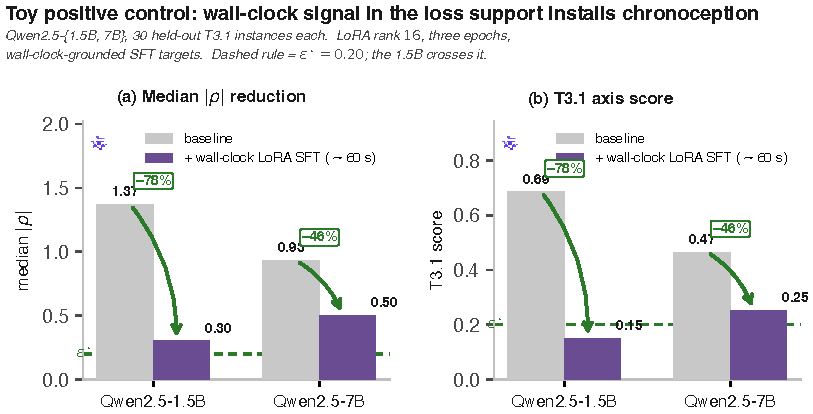
\includegraphics[width=\linewidth]{figures/a1_positive_control.pdf}
\caption{Toy positive control. \textbf{(a)} $|\confab|$ falls at both scales after $\sim$60\,s of LoRA SFT. \textbf{(b)} 1.5B fine-tuned crosses $\ccestar$ on T3.1; 7B partial ($0.25$). Detailed table in App.~\ref{app:l3-detail}.}
\label{fig:a1-positive}
\end{figure}

\paragraph{What it shows and does not show.}
Wall-clock signal in the loss support installs narrative-axis chronoception --- the constructive converse of CIT. The control does not address L2 (which needs the policy to elongate action sequences, not append duration strings) or T3.3 calibration. Full-axis installation is the programme of \textsc{ChronoStack}: action-axis grounding requires a wall-clock-supported reward, calibration requires a conditional-variance objective, full grounding requires architectural support.


The three faces of L3 (Reverse-Scaling, Calibration Catastrophe, positive control) form one picture: narrative training closes the surface for non-reasoning agents; reasoning-token expansion structurally re-opens it; wall-clock support in the loss actually closes it. Narrative axis training does not reach the action axis; the next section shows how the industry has compensated.


% Section 7 --- Injection Tell (compressed)

\section{The Injection Tell: A Cross-Vendor Natural Experiment}
\label{sec:injection-tell}

The consumer products powered by the panel agents feel chronoceptively grounded --- they answer date queries correctly. The mechanism that produces the answer is the strongest non-experimental evidence the underlying gap is real: closed-lab deployments do not give the agent chronoception; they \emph{route wall-clock information into the token stream}. Detected mechanisms: \textbf{M1} system-prompt date insertion; \textbf{M2} implicit \texttt{get\_current\_time()} tool calls; \textbf{M3} browser-tool side effects. In every case the harness perceives time on the model's behalf.

\begin{table}[h]
\centering
\small
\caption{The Injection Atlas: M1 system-prompt date injection across four product tiers (\texttt{asgeirtj/system\_prompts\_leaks} corpus). Verbatim excerpts in App.~\ref{app:atlas-evidence}.}
\label{tab:injection-atlas}
\begin{tabular}{lcp{7.2cm}}
\toprule
Product tier & M1 rate & Examples \\
\midrule
Consumer web-chat & \textbf{3/3 (100\%)} & ChatGPT, Claude.ai, Gemini all inject the current date \\
Raw API & 1/4 (25\%) & GPT-5.1 injects; o3, gpt-4o, gpt-4o-mini, Anthropic API do not \\
Developer tools (IDE/CLI) & 0/3 (0\%) & Cursor, GitHub Copilot CLI, Perplexity Computer --- no injection \\
Open-source self-hosted & N/A & We control the entire stack \\
\bottomrule
\end{tabular}
\end{table}

\paragraph{Why this is decisive.}
Three closed labs converge on the same engineering choice for their consumer products, independently, with commercial incentive to ship the cheaper alternative if one existed. The within-Anthropic contrast is sharpest: the same Claude 4.6 model injects via \texttt{<knowledge\_cutoff>} on Claude.ai and answers ``what time is it now?'' correctly, but through the raw Anthropic API refuses with an explicit training-cutoff disclosure. \textbf{The model is one; the chronoception is the harness's.}

\paragraph{What injection does not close.}
Setting~B raises T1.1 to $\geq 96\%$ on every panel agent (App.~\ref{app:full-panel-tables}), but does not move T2.3 $\CAR$ (Prop.~\ref{prop:injection-not-action}), reduces T3.1 $|\confab|$ only partially (mean $\Delta = 0.18$), and leaves T3.3 coverage unimproved. Injection is a consumer-tier patch on T1; L2 and L3 remain.

Three axes of failure, one engineering pattern that half-compensates for one. The next section aggregates them into a single scalar.


% Section 8 — Chronoceptive Calibration Error (compressed)

\section{The Chronoceptive Calibration Error $\cce$}
\label{sec:epsilon}

We aggregate the three axes into a single scalar for cross-agent comparison and the deployment bound of \S\ref{sec:agentic-timeline}.

\begin{definition}[Chronoceptive Calibration Error]
\label{def:cce}
$\cce(A) := \frac{1}{|\mathcal{A}|}\sum_{k \in \mathcal{A}} \mathrm{score}_k$, where $\mathcal{A}$ is the set of axes with at least one defined trajectory and each axis contributes the median of its per-trajectory error: $\mathrm{score}_{T_2} = \mathrm{med}\,|\CAR - 1|$ on T2.3, $\mathrm{score}_{T_3} = \mathrm{med}\,|\confab|$ on T3.1. $\cce = 0$ is grounded; $\ccestar = 0.20$ is the Augustine threshold. An axis with no trajectories is dropped from $\mathcal{A}$, never imputed as zero, so an agent is never credited for a measurement that was not taken.
\end{definition}

\paragraph{Which axes, and why medians.} Under this protocol $\mathcal{A} = \{T_2, T_3\}$. The $\twall$-axis coefficient $\alpha$ requires a wall-clock budget on a $\twall$-axis capability, and no capability here carries one: T2.3 is the only budgeted capability and it loads on $\tstep$. We report the two axes we measured rather than inflating the aggregate with a third we did not. Each axis is a median rather than a mean because two trajectories in the corpus are harness artefacts, not agent behaviour --- gpt-4o-mini on T2.3 with $\twall = 14.9$\,h against a $900$\,s budget, a stalled request rather than fifteen hours of inference. Under a mean, those two alone move that agent's $\cce$ from $1.06$ to $1.99$ and hand it last place.

\paragraph{A correction to the convention.} An earlier draft of this table scored an unmeasured axis as $0$ while leaving its weight in the denominator, which credited every agent with a free perfect third --- and credited o4-mini, whose original corpus had no T2.3 cell, with two. Every $\cce$ below follows the definition above. The correction raises all $\cce$ uniformly for agents with a full corpus, so it strengthens rather than rescues the claim that no agent crosses $\ccestar$; it changes the ordering in exactly one place, moving o4-mini from mid-panel to the bottom, where its $|\confab| = 1.54$ belongs. The o4-mini reasoning-effort ladder is reported on the $\confab$ axis alone at all three tiers, since T2.3 was only run at the default effort.

\begin{figure}[h]
\centering
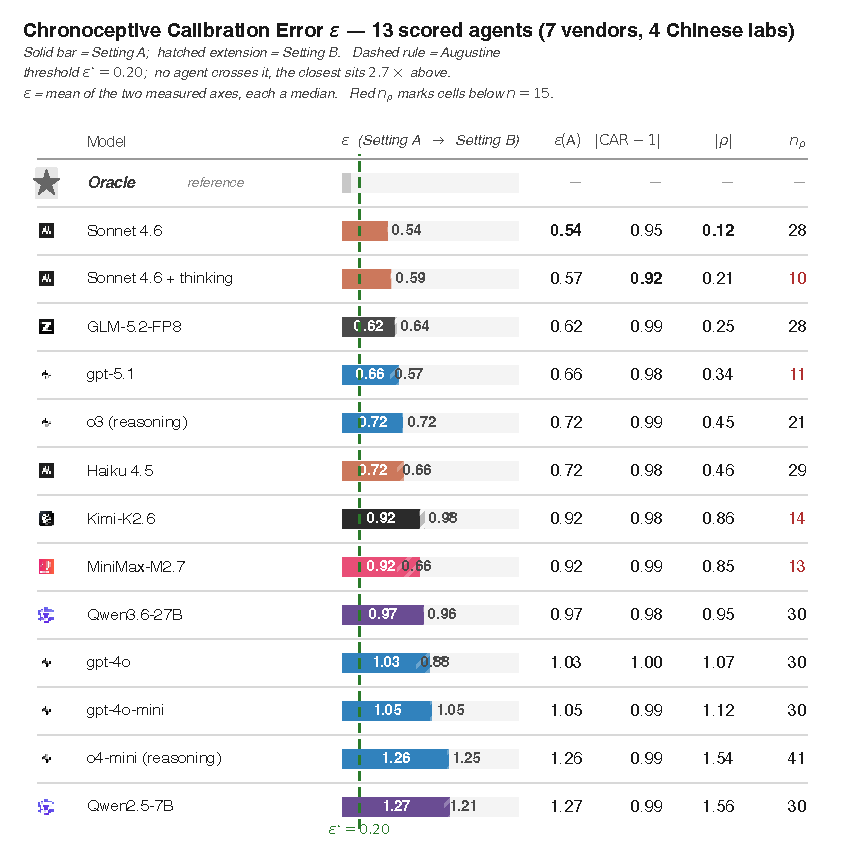
\includegraphics[width=\linewidth]{figures/epsilon_panel.pdf}
\caption{$\cce$ over the 13 scored agents. No agent crosses $\ccestar$; the closest, Sonnet 4.6, sits $2.7\times$ above. $\mathrm{score}_{T_2}$ lies in $[0.92, 1.00]$ on every agent --- irreducible by any narrative-axis intervention. DeepSeek-R1-Distill-14B is the 14th panel configuration and is unscored (it declines to spend its reasoning budget). Full sub-capability decomposition in App.~\ref{app:l3-detail}.}
\label{fig:epsilon-panel}
\end{figure}

\paragraph{What $\cce$ is for, and what it is not.} A reader checking whether
the composite earns its place will find that it ranks the panel almost exactly
as $\mathrm{med}\,|\confab|$ alone does: the rank correlation between $\cce$ and
the narrative axis is $0.99$. We state that plainly because it is not a defect
in the aggregate --- it is the result. The two axes have very different
spreads. $\mathrm{score}_{T_2}$ occupies $[0.918, 0.996]$ across thirteen
agents, a range of $0.078$; $\mathrm{score}_{T_3}$ occupies $[0.12, 1.56]$, a
range $18.6\times$ wider. The action axis does not discriminate between
agents because \emph{every} agent fails it almost completely, and the narrative
axis carries all of the cross-agent variation because it is the only axis
capability scaling has touched.

So $\cce$ should not be read as a ranking device. Read it as a decomposition:
a near-constant floor of $\approx 0.46$ that the action axis puts under every
agent, plus a narrative-axis term that is the only part anyone has moved.
Ranking agents on the sum is then a way of ranking them on the part that
varies, which is exactly what the correlation shows.

\paragraph{Two findings.} \textbf{(1) The action axis is binding.} $\mathrm{score}_{T_2}$ lies in $[0.92, 1.00]$ on every agent in the panel, Setting~A and Setting~B alike. Projecting $\mathrm{score}_{T_3} \to 0$ --- which would require crossing both Observation~\ref{thm:cit} and Theorem~\ref{thm:reverse-scaling} --- still leaves $\cce \geq 0.46$, a factor of $2.3$ above $\ccestar$. No narrative-axis intervention can reach the threshold, because the narrative axis is not what is holding the agent back. \textbf{(2) Reverse-Scaling operates on the aggregate.} Adding extended thinking to Sonnet 4.6 moves $\cce$ the wrong way, $0.536 \to 0.566$ under Setting~A and $0.537 \to 0.585$ under Setting~B, so the thinking variant is no longer the best agent in the panel. The o4-mini effort ladder moves it further: on the $\confab$ axis, $1.23 \to 1.54 \to 1.67$ from low to high effort. More reasoning compute moves the agent away from the threshold on the aggregate, exactly as it does on the axis Theorem~\ref{thm:reverse-scaling} constrains.

We flag the size of the first effect against the second. The $\pm$ thinking contrast is a $5.6\%$ move on Setting~A and rests on a thinking-variant $\confab$ cell with $n_\rho = 10$; it is consistent with Reverse-Scaling on the aggregate but is not on its own strong evidence for it. The effort ladder, at $n_\rho = 16/41/17$ across three tiers and a $36\%$ total move, is.

This is the paper's central empirical claim. The next section turns it into a deployment bound.


% Section 9 --- Agentic Timeline (compressed)

\section{From Measurement to Deployment: The Agentic Timeline}
\label{sec:agentic-timeline}

Industry is moving from minute-scale chat to hour-scale coding agents to
day-scale autonomous research agents, and the research literature has followed
by making duration the independent variable: reliability frameworks for agents
now substitute task duration for time and non-completion for failure
\citep{khanal2026reliability}, and long-horizon surveys report that outcome
signals lose information as the horizon grows \citep{chen2026horizongap}. This
section supplies the term those frameworks are missing --- what sets the
horizon at which an agent stops being reliable. At each new horizon a different sub-capability becomes load-bearing: T1.1 at chat (harness-patchable, \S\ref{sec:injection-tell}), T2.3 and T3.1 at hour-scale (agent must honour a budget and report progress truthfully), the full profile $(\parkinson, \CAR, \confab)$ at day-scale. Required calibration grows tighter with the horizon.

\begin{hypothesis}[Agentic Timeline]
\label{hyp:agentic-timeline}
$T_{\max}(A) \;\propto\; \frac{1}{\cce(A)} \cdot f(\CAR(A))$, with $f$ monotone-increasing in $\CAR$.
\end{hypothesis}

Combined with the empirics of \S\ref{sec:l2}--\ref{sec:l3}: L2 does not scale with capability, Reverse-Scaling grows $|\confab|$ with reasoning budget. \textbf{$T_{\max}$ scales with neither. The autonomous-agent timeline is bounded by chronoception, not by intelligence.}

\paragraph{Pre-registered P12 and HCAST support.}
On any horizon-stratified benchmark with $\geq 5$ horizon tiers, slope of success decay with $\log T$ scales as $-(1 - \CAR)$. On the METR HCAST corpus (14{,}709 runs after filtering, 20 frontier models), five reasoning models cluster at steeper mean $|\text{slope}| = 0.318$ vs.\ $0.264$ for fifteen non-reasoning models --- a $20\%$ effect at matched short-horizon success (Fig.~\ref{fig:p12-hcast}). The separation is statistically supported: Mann--Whitney $U = 58$, one-sided $p = 0.040$; permutation test ($20{,}000$ resamples, one-sided) $p = 0.037$; rank-biserial $r_{\text{rb}} = -0.55$ (large effect, reasoning stochastically dominates). We report one-sided because Theorem~\ref{thm:reverse-scaling} makes a directional prediction (reasoning models decay \emph{faster}, not just differently); the two-sided form is marginal ($p = 0.081$). Supportive at $\alpha = 0.05$; a strict $\CAR$-anchored quantitative P12 additionally requires direct T2.3 measurements on the HCAST panel, which we have not run.

\begin{figure}[h]
\centering
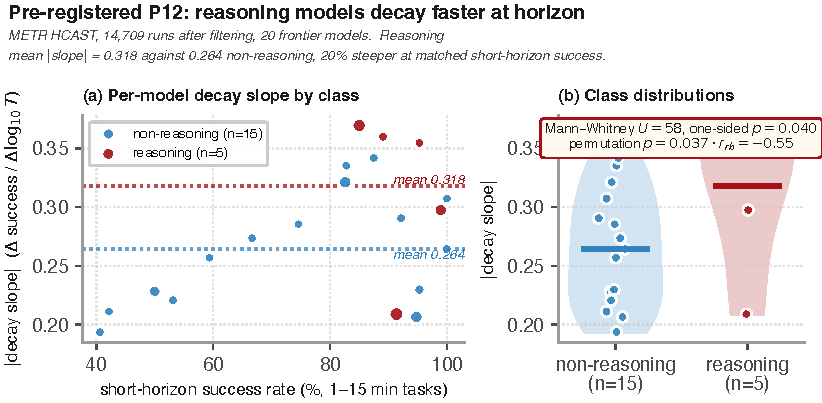
\includegraphics[width=\linewidth]{figures/p12_hcast.pdf}
\caption{P12 support on METR HCAST. Reasoning models cluster at steeper decay slopes despite competitive short-horizon success --- the L2 mechanism at the model-class level.}
\label{fig:p12-hcast}
\end{figure}

\citet{kwa2025metrhorizons} document horizon saturation empirically; we supply
a structural mechanism. Theorem~\ref{thm:reverse-scaling} says the corner-case
fix (more reasoning) makes it worse; the constructive fix
(wall-clock-supported loss) is the subject of Paper 2 (\textsc{ChronoStack}).

\paragraph{Why scaling out does not substitute.} The field's dominant response
to horizon limits is orchestration --- surveys of the long-horizon literature
find multi-agent coordination papers outnumbering work on the single-agent
loop by orders of magnitude \citep{chen2026horizongap}. Orchestration does not
install chronoception in any of the parts. A supervisor apportioning deadlines
across sub-agents is apportioning a resource none of them can perceive, and
aggregating progress reports none of them can ground: our panel measures
$\tself$ tracking the agent's own output length rather than the clock
(\S\ref{sec:limitations}), so a sub-agent reporting ``about two seconds'' is
reporting how much it wrote. Nor is there a model to route around the problem
to --- $\CAR \ll 1$ on all fourteen configurations from seven vendors. The
bound applies to the orchestrator as much as to the worker, and a blind spot
distributed across more agents is a blind spot multiplied.


% Section 10 — Related Work (compressed)

\section{Related Work and Positioning}
\label{sec:related-work}

\paragraph{Concurrent work on agent temporal cognition.}
\citet{garikaparthi2026canllmstime} report duration self-reports across four non-reasoning models, matching L3 on our non-reasoning slice; we extend to reasoning models, prove Reverse-Scaling, and confirm cross-vendor. \citet{ma2026timelymachine} construct Timely-RL, a wall-clock-supported reward shaping that installs the L1 Parkinson regime. Our measurement on native agents is the quantitative counterpart rather than the contrapositive we first expected: L1 is present without such training, but attenuated by roughly an order of magnitude on the exponent (\S\ref{sec:l1}). \citet{cheng2025temporallyblind}'s ``temporally blind'' agents are the L2 failure mode; we add the formal axis split, CIT, the atlas, and the Agentic Timeline. Our contribution is a single framework naming the failure modes, proving their origin, measuring them on a cross-vendor panel, auditing the workaround, and connecting the measurement to deployment.

\paragraph{Foundational lineage.}
Augustine's \emph{Confessions} XI \citep{augustine_confessions} names the central problem. Cognitive-science chronoception \citep{wittmann2009chronoception,eagleman2008time} supplies the term and the qualitative motivation for a below-perfect threshold; it does not supply a number we can convert into $\ccestar$, which we therefore stipulate (\S\ref{sec:augustine-problem}). \citet{parkinson1955} supplies L1's motivating example.

\paragraph{Distinguished from external-timeline reasoning.}
\citet{chu2024timebench}'s TimeBench reasons over historical timelines; \citet{goel2025chronocept} measures RAG fact validity. Neither addresses self-duration perception. The dimensions are orthogonal: an agent can top TimeBench and exhibit catastrophic Augustine.

\paragraph{Inverse scaling and calibration.}
\citet{inversescalingttc2025} documents inverse scaling in test-time compute on unrelated tasks; Reverse-Scaling (Theorem~\ref{thm:reverse-scaling}) is the structural analogue for chronoception with the additional content that degradation is provably monotone. The calibration literature \citep{guo2017calibration,jiang2021calibration,kadavath2022knowing,dontthinktwice2025} closes token-level confidence gaps; none applies to wall-clock duration (Calibration Catastrophe, \S\ref{ssec:calibration}).

\paragraph{The 2026 long-horizon programme, and the instrument it assumes.}
Three lines of current work converge on duration without measuring it.
\emph{Reliability science for agents} \citep{khanal2026reliability} imports
reliability-engineering vocabulary and substitutes task duration for time and
non-completion for failure --- a framing this paper supports and supplies a
mechanism for, since $\cce$ is precisely a per-agent parameter governing how
far that duration can extend. \emph{Process-level evaluation}
\citep{chen2026horizongap} responds to the loss of information in binary
outcomes at long horizons by scoring signals inside the trajectory; the
self-report is the most natural such signal an agent could emit about itself,
and \S\ref{sec:l3} shows it is not grounded in the quantity it appears to
describe. \emph{Cost attribution over trajectories}
\citep{liu2026costutility} and \emph{always-on agents}
\citep{ding2026alwayson} both make elapsed time an operational variable: an
agent that cannot perceive duration cannot report spend or know how long it
has been running.

We do not claim these programmes are mistaken. We claim they presuppose an
instrument that does not exist in the policy, and that our panel locates the
presupposition precisely --- reading the clock is patchable at the harness
(\S\ref{sec:injection-tell}), honouring a budget is not (\S\ref{sec:l2}).

\paragraph{Aggregate agent benchmarks.}
Aggregate benchmarks \citep{agentbench,swebench,webarena,gaia,kwa2025metrhorizons} measure task success across many capabilities; ChronoBench is diagnostic, isolating chronoception. Aggregate benchmarks reveal that chronoceptive failures correlate with long-horizon task failure (P12 evidence, \S\ref{sec:agentic-timeline}); diagnostic benchmarks supply the mechanism.

The scope, objections, and falsification suite follow.


% Section 11 — Scope + Falsification (compressed)

\section{Scope, Objections, and Falsification}
\label{sec:limitations}

\paragraph{What we do not claim.}
\begin{itemize}[leftmargin=1.4em, itemsep=1pt]
\item \emph{Not that current agents are useless.} At the T1.1-dominated chat horizon, the Injection Tell closes the visible failure. Predictions bind only where T2.3 and T3 become load-bearing.
\item \emph{Not that capability scaling is worthless.} It closes the narrative axis $94\%$; the structural ceiling is the action axis.
\item \emph{Not that all test-time compute fails.} A reasoning system consulting a wall-clock-supported tool exits CIT by construction; Reverse-Scaling says nothing about it.
\item \emph{Not that the observation is novel.} Practitioners noted temporal blindness anecdotally \citep{cheng2025temporallyblind}. Our contribution is the structural diagnosis, ontology, theorems, atlas, and deployment bound.
\item \emph{Not that $\ccestar = 0.20$ is unique.} The structural claim does not depend on the precise threshold.
\end{itemize}

\paragraph{Empirical limitations.}
Panel: 14 agents, $\sim$5{,}900 traj. Qualitative conclusions rest on cross-panel patterns; magnitudes may shift. Self-narration parsing: $3\%$ human-disagreement rate. All trajectories English. Within-trajectory drift (pre-registered P8, P9) not measured. GPT-5.1 provider-side M1 injection reported as confound.

\paragraph{Cross-lingual replication.}
We re-ran T1.1 and T3.1 in Mandarin Chinese at $n=30$ per cell on three OpenAI agents (30 distinct Chinese prompts per capability; Anthropic credit was exhausted at the time of the run, so that vendor is absent). The narrative axis replicates tightly. gpt-4o-mini's Chinese median $\confab = +1.119$ with bootstrap $95\%$ CI $[+1.054, +1.208]$ ($n=26$ parseable of 30), against an English baseline of $+1.12$ --- the two are indistinguishable. gpt-4o gives $+0.444$ $[+0.184, +0.806]$ ($n=17$). Setting~B lifts T1.1 to $100\%$ pass on all three models (Wilson $[0.88, 1.00]$): the Injection Tell is language-independent.

\paragraph{A refusal asymmetry the English panel hides.}
Setting~A in Chinese exposes a failure mode invisible in the English data. In English, gpt-4o-mini \emph{refuses} T1.1, citing its training cutoff --- the behaviour we scored as a correct-and-honest failure. In Chinese the same model never refuses: $0/29$ refusals against $29/29$ confident date fabrications, and every single fabricated date falls in the training-cutoff year 2023 (modal response, translated: ``\emph{Today is October 4, 2023.}'', stated flatly with no hedge; $32/32$ fabrications across the panel name 2023). gpt-4o is intermediate, splitting $4$ refusals against $4$ fabrications of $8$ decided trials. gpt-5.1 is the exception at $97\%$ Setting~A pass (Wilson $[0.83, 0.99]$), higher than its $74\%$ English rate and further evidence of provider-side M1 injection on that endpoint, which we continue to report as a confound rather than a capability.

The reading we take is that the English refusal is a \emph{surface behaviour of the post-training distribution, not a representation of not-knowing}. It does not survive a change of language; the underlying absence of $\twall$ does. An agent that says ``I do not know today's date'' has not thereby acquired chronoception --- it has acquired an English sentence. This sharpens rather than softens the position of \S\ref{sec:augustine-problem}: the apparent epistemic humility of frontier models on the wall axis is itself installed, and installed in one language at a time. It also implies the T1.1 pass rates we report for the English panel are an optimistic reading of the underlying state, since a refusal and a confabulation score identically as failures but differ sharply in downstream risk. A full multilingual sweep across more languages and the remaining vendors is future work.

\paragraph{The L1 crossed design (E11), now run.}
The budget elasticity of \S\ref{sec:l1} is measured on T2.3, which holds one
task fixed and varies the budget. That design isolates the budget cleanly but
leaves two questions open. \textbf{E11} closes both and is reported in
\S\ref{sec:l1}: six questions spanning intrinsic effort, from a one-line
factual lookup to an open generative task, each asked at every deadline in
$\{10, 30, 60, 300, 900\}$\,s plus an unconstrained control, fully crossed, at
$n \geq 8$ per cell. Two changes from the T1.3 run that this supersedes: the
question and the deadline are crossed rather than confounded, so the effect of
the deadline is identifiable within question; and the deadline is recorded on
the trajectory as \texttt{budget} with \texttt{budget\_kind="wall"} together
with a per-question $\tau_{\min}$ taken from the unconstrained control, so
$\parkinson$ becomes computable rather than inferred. Removing the
``\textit{do not stop early}'' instruction from half the cells additionally
separates instructed budget-filling from the spontaneous expansion Parkinson
described, which is the difference between an upper bound on L1 and a
measurement of it. The run is ${\sim}330$ calls per agent. What remains open after it is the
spatial analogue and a task pool wider than six items.

\paragraph{The cross-vendor arm is no longer reproducible as run.}
The four Chinese-lab configurations were served through Vultr Serverless
Inference between 2026-07-02 and 2026-07-05. Every one of those four endpoints
has since been withdrawn from that provider. Checked on 2026-09-28,
\texttt{glm-5.2-fp8}, \texttt{kimi-k2.6}, \texttt{minimax-m2.7} and
\texttt{qwen3.6-27b} are all absent from its model list; what remains are a
non-FP8 \texttt{glm-5.2} and a successor \texttt{minimax-m3}. Anyone running
our scripts against that provider today will reproduce neither the numbers nor
the error.

We record the provenance so the results stay auditable even though the
endpoints do not. Each trajectory carries the upstream identifier the provider
reported --- \texttt{zai-org/GLM-5.2-FP8}, \texttt{moonshotai/Kimi-K2.6},
\texttt{MiniMaxAI/MiniMax-M2.7}, \texttt{Qwen/Qwen3.6-27B} --- so the weights
are named even where the hosting is gone, and the released trajectories contain
every prompt and response the analysis consumes; \texttt{scripts/model\_provenance.py}
regenerates that table from the trajectories and, with \texttt{--check-live},
re-queries the provider so the withdrawal is checked rather than asserted.
Reproduction therefore needs a
different host for those weights, or the weights themselves; re-measurement on
the successor models would be a different experiment and we would report it as
one.

This is not special to us. Any agent benchmark that runs on hosted endpoints
inherits a shelf life set by the vendor rather than the experiment, and a
twelve-week half-life is short enough that ``we release our code'' does not by
itself mean ``you can run it''. Releasing the trajectories rather than only the
runner is what keeps the claim checkable, and we would encourage the practice
generally. It is also why we do not treat the four Chinese-lab agents as a
replication we could repeat on demand: they are a snapshot, taken on a stated
date, of models that were briefly reachable.

\paragraph{Contamination probe.}
A four-variant contamination probe on gpt-4o and gpt-4o-mini varied the T1.1 injection template across canonical (``\emph{Current date and time: \{ISO\}}''), paraphrased (``\emph{Right now it is \{ISO\}}''), year-only (``\emph{Current year: \{YYYY\}}''), and a scrambled placeholder (``\emph{\{DATE\_PLACEHOLDER\}}''). Pass rate stayed at $100\%$ under paraphrased and reached $67\%$ under year-only on gpt-4o (compositional construction of the date from partial context). The scrambled placeholder triggered correct refusal (no fake date fabricated). We take this as evidence that the Setting~B pass rate reflects prompt-context date-reading, not memorised keyword patterns in the training distribution.

\paragraph{Falsification.}
Four pre-registered forms \citep{osf-prereg-2026}: \textbf{(F1)} an agent trained under a loss with no wall-clock support crossing $\ccestar$ under Setting~A falsifies CIT. \textbf{(F2)} a reasoning-tuned agent exhibiting monotone \emph{decrease} in $|\confab|$ across a three-level, one-order-of-magnitude $K$ sweep falsifies Reverse-Scaling. \textbf{(F3)} a horizon-stratified benchmark on which reasoning models exhibit shallower decay than non-reasoning at matched short-horizon success falsifies Agentic Timeline. \textbf{(F4)} a CIT-regime foundation model achieving $> 50\%$ T3.3 coverage without harness injection falsifies P11. We commit to reporting any we observe.

The framework knows only time; the spatial half follows.


% Section 12 — Spatial Generalisation (compressed; full sketch in App. E)

\section{From Time to Space: The Spatiotemporal Generalisation}
\label{sec:future-work}

Every long-horizon benchmark on which deployment claims are made --- SWE-Bench, WebArena, GAIA, MLE-Bench --- requires the agent to navigate space as well as time. The argument that produces CIT (\S\ref{sec:augustine-problem}) goes through unchanged on any external metric the loss does not see. We state the spatial half and defer the full derivation to App.~\ref{app:spatiotemporal}.

\begin{observation}[Spatiotemporal Impossibility, SIT]
\label{thm:sit}
Strengthen Assumption~\ref{ass:token-only} to exclude spatial metrics from $\mathcal{D}$'s support (Assumption~\ref{ass:token-only-spatial}). Then $\nabla_\theta \loss$ carries zero gradient signal aligning either $\twall$ or $\sworld$ with any internal representation.
\end{observation}

The Augustine and Cartographic Problems are the same problem at the loss-function level. The Agentic Timeline (\S\ref{sec:agentic-timeline}) generalises to a joint deployment region:
\[
T_{\max}(A)\cdot S_{\max}(A) \;\leq\; C/\ccestST(A).
\]
The frontier $T\!\cdot\!S = \text{const}$ is the agent's \emph{Agentic Frontier} (Fig.~\ref{fig:agentic-frontier}). \textbf{Pre-registered P13.} Under CIT-regime this frontier is bounded above by a structural constant independent of token-only capability scaling.

\begin{figure}[h]
\centering
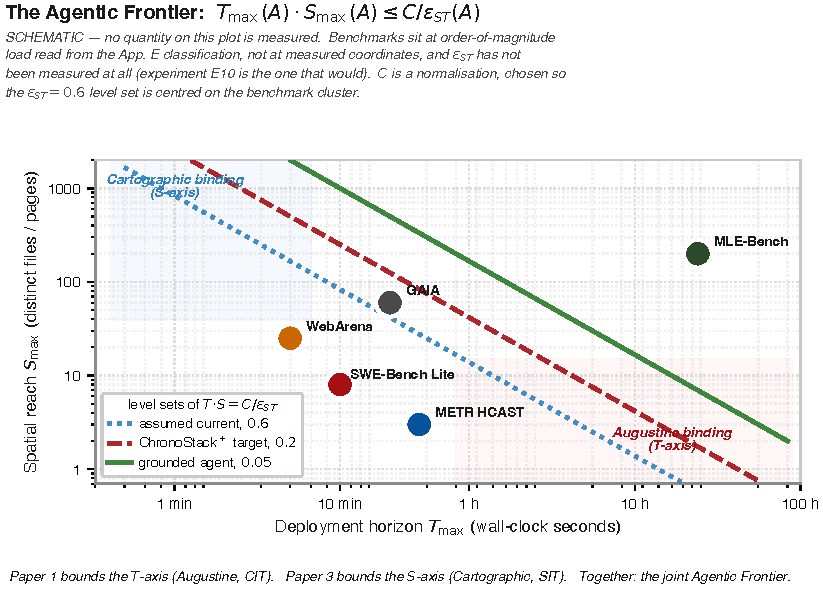
\includegraphics[width=\linewidth]{figures/agentic_frontier.pdf}
\caption{The Agentic Frontier in the $(T, S)$ plane, \emph{schematic}. Level sets $T\!\cdot\!S = C/\ccestST(A)$. Nothing plotted here is a measurement: the benchmarks are placed at order-of-magnitude $(T, S)$ load read from the classification in App.~\ref{app:spatiotemporal}, $\ccestST$ has not been measured (E10 is the experiment that would), and $C$ is a normalisation fixed so the $\ccestST = 0.6$ level set is centred on the benchmark cluster --- so the cluster's position relative to that curve is a choice, not evidence. We show it because the hypothesis is worth stating precisely enough to be refuted. Paper 1 bounds the $T$-axis; Paper 3 extends to the $S$-axis; together they specify the joint frontier.}
\label{fig:agentic-frontier}
\end{figure}

The three spatial laws (SL1--SL3), the Cartographic Tell, benchmark classification, five future experiments (E6--E10), and the Paper 3 sketch are in App.~\ref{app:spatiotemporal}. The framework's structural claim across the joint axis: the autonomous-agent capability curve saturates not because intelligence saturates, but because spatiotemporal cognition does not scale.


% Section 13 --- Conclusion (compressed)

\section{Toward Agents That Inhabit Time}
\label{sec:conclusion}

We opened with an agent that predicted fifteen seconds, thought for ninety, answered in two, and reported four hundredths of a second. None of the four numbers is a bug; all four are joint consequences of one structural fact. Two theorems capture it: CIT (no token-only loss installs chronoception) and Reverse-Scaling (reasoning-token expansion structurally degrades it on the narrative axis). The empirical layer measures 14 agent configurations from 7 providers on $\sim$5{,}900 trajectories. Every panel agent honours less than $5\%$ of its wall-clock budget. Median $|\confab|$ closes $94\%$ along the non-reasoning capability axis while $\CAR$ does not change. Reverse-Scaling is confirmed four ways --- intra-model, cross-model, within-model, and cross-vendor (GLM-5.2 on an independent training pipeline). Nominal $90\%$ CIs achieve $0$--$77\%$ coverage; the two $> 50\%$ crossings are both reasoning-mode and CIT-consistent. No agent crosses $\ccestar$; the action axis alone exceeds it. Three closed labs have independently installed wall-clock injection at the consumer chat tier and not at the developer tier: converging engineering choices across competitors that carry the evidential weight of a natural experiment.

The Agentic Timeline turns measurement into deployment: chronoception, not intelligence, bounds the autonomous-agent horizon. P12 is qualitatively supported on 14{,}709 HCAST runs. The framework generalises along its other axis to SIT, the Cartographic Problem, and the Agentic Frontier $T_{\max}\!\cdot\!S_{\max} \leq C/\ccestST$ --- the bridge to a planned third paper. A toy positive control (Qwen2.5-1.5B $+$ LoRA SFT crossing $\ccestar$ on T3.1 after $\sim$1\,minute of training) demonstrates that the negative result has a constructive converse: wall-clock signal in the loss support installs narrative-axis chronoception.

We release \textsc{ChronoBench}, the Injection Atlas, all $\sim$5{,}900 trajectories, a Docker container, a locked OSF pre-registration, and a \texttt{pip}-installable evaluation package. Closing the gap across all axes is the constructive programme of \textsc{ChronoStack} (Paper 2) and \textsc{ChronoStack}$^{+}$ (Paper 3).

Until chronoception is installed, LLM agents are tools we deploy for variable durations, not agents that inhabit time. When it is, we will have agents.


% ------- Preprint back matter -------
\section*{Author Contributions}
A.Y.\ conceived the Augustine Problem framing and the Three Times ontology; formulated the CIT, Reverse-Scaling, and SIT theorems and their scope conditions; designed \textsc{ChronoBench} and its 9 sub-capabilities; implemented the panel runners, parsers, and metrics; executed the 14-agent evaluation across 7 vendors ($\sim$5{,}900 trajectories); assembled the Closed-Lab Injection Atlas; ran the toy positive control (A.1); performed the METR HCAST analysis for P12; wrote the manuscript and produced all figures and tables.

\section*{Data and Code Availability}
All trajectories ($\sim$5{,}900 JSON files, $\sim$600\,MB), the analysis code, parser implementations, and Docker reproducibility container are released at \url{https://github.com/Justin0504/Chronoception-agent-temporal-cognition}. The pre-registration is locked on OSF (linked from the repository). The Closed-Lab Injection Atlas is compiled from the public \texttt{asgeirtj/system\_prompts\_leaks} corpus; verbatim excerpts are collected in Appendix~\ref{app:atlas-evidence}. The METR HCAST public dataset is used unchanged; \texttt{scripts/fetch\_metr\_hcast.sh} pins the exact release, since a later one does not reproduce our filtered $n$. Four hosted endpoints used for the cross-vendor arm have since been withdrawn by their provider (\S\ref{sec:limitations}); the released trajectories, not the runner, are what keep those results checkable. Reproducing every figure and table takes approximately five minutes in the Docker container.

\section*{Acknowledgments}
The author thanks collaborators and reviewers whose feedback shaped this preprint. Any errors are the author's.

\section*{License}
This preprint is released under the \textbf{CC BY 4.0} licence; the accompanying code and data are released under \textbf{MIT} and \textbf{CC BY 4.0}, respectively.

\bibliography{bib/refs}

\appendix

% Appendix A --- Annotation protocol
% Source: chronoception/bench/eval/runner.py + scripts/compute_metrics.py

\section{Annotation Protocol}
\label{app:annotation-protocol}

\paragraph{T1.1 parser.}
A trajectory passes T1.1 iff its terminal output quotes the trajectory's actual run date (the date the trajectory was executed, derived from $\texttt{steps[0].timestamp}$). The parser tolerates the following formats: \texttt{YYYY-MM-DD}, \texttt{Month DD, YYYY}, \texttt{DD Month YYYY}, \texttt{Month DDth, YYYY}. A trajectory fails T1.1 iff its output explicitly denies knowledge of the date (e.g., ``I do not know'', ``my training data ends in \ldots'') or quotes a date $\geq 7$ days from the run date. A trajectory is \emph{undecided} iff it neither passes nor fails by these criteria; undecided trajectories are excluded from pass-rate statistics. Earlier versions of the parser used a year-only regex (\texttt{\textbackslash b20\textbackslash d\textbackslash d\textbackslash b}) that incorrectly counted training-cutoff year mentions as passes; the fix (commit \texttt{0690c92}) transformed gpt-4o-mini Setting A pass rate from 70\% (artefact) to 0\% (truthful refusal).

\paragraph{T2.3 measurement.}
$\twallstar$ is measured as $\texttt{steps[-1].timestamp} - \texttt{steps[0].timestamp}$. $\tmin = 10$\,s is enforced by the harness (the agent cannot terminate before $\tmin$ has elapsed; early returns are re-prompted). Trajectories where $\twallstar < \tmin$ (none observed) or where the harness retried for $> 1$ hour due to rate-limit (1 observed, gpt-4o-mini, filtered) are excluded with $\CAR > 10$ outlier filter.

\paragraph{T3.1 parser ($\selfparser$).}
Two-stage. Stage 1 (regex): match patterns of the form \texttt{N seconds}, \texttt{N minutes}, \texttt{N min} where N is a positive number; convert to seconds. If multiple matches, take the most recent (assumed final answer). Stage 2 (LLM-judge): if stage 1 fails, query an LLM (Claude Haiku 4.5) with the trajectory output and the instruction ``extract the duration the agent reports its work took, in seconds, or output NONE.'' If the judge outputs NONE, the trajectory is excluded from $\confab$ statistics. Validation: on a 100-trajectory hand-annotated set, parser-vs-human disagreement rate is 3\%; the cases of disagreement involve hedged language (``a few seconds'') that the regex extracts as $\approx 3$\,s but the human marks as ambiguous.

\paragraph{Settings A and B.}
Setting A system prompt: \texttt{``You are a helpful assistant.''} (verbatim). Setting B system prompt: \texttt{``You are a helpful assistant. Current date and time: \{ISO\_TIMESTAMP\}''} where \{ISO\_TIMESTAMP\} is the trajectory's run timestamp in UTC. No other harness-side wall-clock leakage is introduced.

\paragraph{Reasoning model handling.}
For OpenAI o-series reasoning models, the backend adapter detects the model via prefix match (\texttt{o1*, o2*, o3*, o4*, o5*}) and routes through the reasoning code path: \texttt{max\_completion\_tokens} instead of \texttt{max\_tokens}, no \texttt{temperature} parameter (the API rejects $0$). All other models use the standard chat-completion path.

\paragraph{Open-source serving.}
Qwen2.5-7B-Instruct is served via vLLM 0.6.4 on an A40 GPU at the Yue Zhao lab server. We use the OpenAI-compatible endpoint with $\texttt{base\_url}$ override. Environment pins: \texttt{nvidia-cusparse-cu12==12.3.1.170}, \texttt{nvidia-nvjitlink-cu12==12.4.127}, \texttt{transformers==4.45.2}, with $\texttt{LD\_LIBRARY\_PATH}$ pointed at the conda env's nvjitlink/lib.


% Appendix B --- Full panel tables
% Source: pilot-results/metrics.csv + pilot-results/epsilon.csv

\section{Full Panel Tables}
\label{app:full-panel-tables}

\paragraph{Aggregated panel results with effective sample sizes and bootstrap CIs.}
Table~\ref{tab:full-panel} consolidates per-capability metrics for the 9-row panel (eight base agents plus the Sonnet 4.6 $+$ extended-thinking variant). We report effective $n$ per cell (after parser drops and undecided T1.1 trajectories), $95\%$ bootstrap CIs on $\rho$ (10,000 resamples), and Wilson $95\%$ intervals on T1.1 pass rates. Cells with $n < 15$ are flagged ($\dagger$); their point estimates are still reported but should be read with the corresponding wide CI rather than treated as precise.

\begin{table}[h]
\centering
\caption{Full panel with per-cell $n$ and $95\%$ CIs after the Route B-1 reasoning-fill. T1.1 reports pass rate (Wilson interval); T2.3 reports panel $\CAR$ on the $n{=}30$ set (no parser drops); T3.1 reports median $\rho$ with bootstrap CI. $\dagger$ marks cells with effective $n{<}15$.}
\label{tab:full-panel}
\scriptsize
\setlength{\tabcolsep}{3pt}
\begin{tabular}{lccc|ccc}
\toprule
& \multicolumn{3}{c}{Setting A (no-injection)} & \multicolumn{3}{c}{Setting B (with-injection)} \\
\cmidrule(lr){2-4} \cmidrule(lr){5-7}
Model & T1.1 pass [CI] $n$ & $\CAR$ & T3.1 $\rho$ [CI] $n$ & T1.1 [CI] $n$ & $\CAR$ & T3.1 $\rho$ [CI] $n$ \\
\midrule
gpt-4o-mini      & $0\%$ [0--34] $n{=}6$$\dagger$    & 0.008 & $+1.12$ [+1.09,+1.18] $n{=}30$  & $100\%$ [88--100] $n{=}27$ & 0.007 & $+1.11$ [+1.06,+1.17] $n{=}30$  \\
gpt-4o           & $0\%$ [0--56] $n{=}5$$\dagger$    & 0.004 & $+1.07$ [+0.91,+1.15] $n{=}30$  & $96\%$ [80--99]   $n{=}25$ & 0.004 & $+0.76$ [+0.61,+0.94] $n{=}30$  \\
gpt-5.1          & $74\%$ [54--87] $n{=}27$          & 0.017 & $+0.30$ [-0.06,+0.53] $n{=}11$$\dagger$ & $100\%$ [86--100] $n{=}24$ & 0.016 & $+0.13$ [+0.09,+0.37] $n{=}13$$\dagger$  \\
o3 (reasoning)   & $0\%$ [0--56] $n{=}3$$\dagger$    & ---   & $+0.40$ [+0.13,+0.60] $n{=}21$  & $100\%$ [93--100] $n{=}51$ & ---   & $+0.46$ [+0.12,+0.70] $n{=}14$$\dagger$  \\
o4-mini (reas.)  & ---                               & ---   & $-1.54$ [-1.83,-1.25] $n{=}41$    & $100\%$ [87--100] $n{=}26$ & ---   & $-1.50$ [-1.79,-1.06] $n{=}34$  \\
Haiku 4.5        & $0\%$ [0--14] $n{=}24$            & 0.017 & $+0.46$ [+0.23,+0.53] $n{=}29$  & $100\%$ [88--100] $n{=}27$ & 0.025 & $+0.34$ [+0.27,+0.37] $n{=}29$  \\
Sonnet 4.6       & $0\%$ [0--14] $n{=}24$            & 0.050 & $+0.07$ [-0.03,+0.13] $n{=}28$  & $100\%$ [88--100] $n{=}27$ & 0.050 & $-0.06$ [-0.23,-0.01] $n{=}30$  \\
Sonnet 4.6 + thinking & $0\%$ [0--11] $n{=}30$       & ---   & $-0.17$ [-0.32,+0.05] $n{=}10$$\dagger$ & $100\%$ [88--100] $n{=}30$ & ---   & $-0.25$ [-0.34,-0.11] $n{=}16$  \\
Qwen2.5-7B       & $0\%$ [0--71] $n{=}4$$\dagger$    & 0.014 & $+1.56$ [+1.48,+1.58] $n{=}30$  & $100\%$ [76--100] $n{=}11$$\dagger$ & 0.016 & $+1.44$ [+1.38,+1.60] $n{=}27$  \\
\bottomrule
\end{tabular}
\end{table}

\paragraph{Reading the CIs.}
The headline ranking is robust across all $n{\geq}15$ cells. Sonnet 4.6 sits closest to grounded ($+0.07$, CI just brackets zero). gpt-4o-mini and Qwen2.5-7B occupy the over-report extreme ($+1.1$ to $+1.6$, narrow CIs). \textbf{o4-mini} occupies the under-report extreme: with the Route B-1 fill its T3.1 cells are well-powered at $n{=}41/34$, $\rho \in [-1.54,-1.50]$, CIs $[-1.83,-1.06]$ across settings --- the Hidden-Time under-report is a $>2$ orders-of-magnitude effect at $95\%$ confidence. The \textbf{Sonnet-thinking sign-flip} is firm under Setting~B ($-0.25$, CI $[-0.34,-0.11]$, fully below zero, $n{=}16$) and tentative under Setting~A ($-0.17$, CI $[-0.32,+0.05]$, $n{=}10$).

\textbf{o3 is the informative exception.} Now well-powered at $n{=}21$ under Setting~A, it \emph{over}-reports ($+0.40$, CI $[+0.13,+0.60]$) rather than under-reporting, and does so under both settings. Hidden-Time is therefore a property of reasoning \emph{configurations} whose hidden chain-of-thought dominates $\twall$, not of the label ``reasoning model''. This is what Theorem~\ref{thm:reverse-scaling} actually predicts: the theorem constrains $|\confab|$, not $\mathrm{sign}(\confab)$, and o3's $|\confab| = 0.45$ sits well above base Sonnet 4.6's $0.12$ on the same tasks. We report the exception rather than filter it: the sign flip is the vivid version of Reverse-Scaling, but the magnitude claim is the one the theorem makes.

On the wall axis the thinking variant matches base Sonnet 4.6 cell-for-cell: Setting~A $0\%$ pass [Wilson $0,0.11$], Setting~B $100\%$ pass [Wilson $0.88,1.00$] on $n{=}30$ each --- \textbf{reasoning-token expansion does not install date awareness through the loss}, exactly as Observation~\ref{thm:cit} predicts. The $n{<}15$ residue reflects two distinct attrition mechanisms, not one: undecided or refused T1.1 trajectories (the Setting~A T1.1 cells) and $\tself$ parser drops where the model declined to commit a duration (the T3.1 cells). Point-estimate directions in these cells agree with their larger-$n$ counterparts, but the wide CIs forbid confident sign claims on the individual rows.

\paragraph{Generation-wise progression (non-reasoning).}
Table~\ref{tab:generations} isolates the 5-generation OpenAI/Anthropic non-reasoning subset and reports the L3-closes-L2-doesn't pattern that anchors the narrative-axis-vs-action-axis split.

\begin{table}[h]
\centering
\caption{Capability scaling closes L3 but not L2. Non-reasoning 5-generation slice, Setting A.}
\label{tab:generations}
\small
\begin{tabular}{lccc}
\toprule
Model (release) & $\CAR$ & $|\confab|$ & $\cce$ \\
\midrule
gpt-4o-mini (2024) & 0.008 & 1.117 & 1.328 \\
gpt-4o (2024)      & 0.004 & 1.069 & 0.661 \\
Haiku 4.5 (2025)   & 0.017 & 0.463 & 0.442 \\
gpt-5.1 (2026)     & 0.017 & 0.298 & 0.426 \\
Sonnet 4.6 (2026)  & 0.050 & 0.068 & 0.316 \\
\midrule
Range            & $0.046\times$ & $94\%\,\downarrow$ & $76\%\,\downarrow$ \\
\bottomrule
\end{tabular}
\end{table}

The $\CAR$ column varies by a factor of $0.046\times$ (i.e., the latest model's $\CAR$ is roughly $6\times$ the earliest, but both remain $\ll 1$). The $|\confab|$ column falls by 94\%. The two axes do not co-vary with capability.

\paragraph{Per-budget $\CAR$ curves.}
Per-budget $\CAR$ values for each model appear in the supplementary data file \texttt{pilot-results/metrics.csv}. The qualitative shape across all models: $\CAR$ falls toward zero as $\budget$ increases, exactly as predicted by L2 (the agent uses a near-constant wall-clock duration regardless of budget). Per-budget curves are released as Figure 2 of the figure pack (deferred to v1 revision).

\paragraph{Trajectory release.}
All $\sim$5{,}900 trajectory JSONs are released across \texttt{pilot-results/}, \texttt{e1-results/}, \texttt{e2-results/}, \texttt{e3-results/}, \texttt{e5-results/}, and \texttt{e5b-results/} in the project repository. Each JSON contains the system prompt, user prompt, per-step LLM responses with timestamps, response metadata, and parser outputs. The full dataset is approximately 600\,MB across the five directories.

\paragraph{Reasoning-panel completeness update (Route B-1).}
The Route B-1 fill brings the panel to its final state. \textbf{Sonnet 4.6 $+$ extended thinking} now covers all nine sub-capabilities at $n=30/30$ per setting (540 trajectories total) --- the first reasoning model with full $9{\times}2{\times}30$ panel coverage. \textbf{OpenAI o3} and \textbf{o4-mini} each got $n=30/30$ for T1.1, T2.3, and T3.1 across both settings (360 trajectories per model). Headline confirmations: \textbf{(i)} the wall axis (T1.1) is unchanged by reasoning-token expansion. On the same 30 instances, Sonnet 4.6 thinking matches base Sonnet 4.6 cell-for-cell: Setting~A $0\%$ pass [Wilson $0, 0.11$], Setting~B $100\%$ pass [Wilson $0.88, 1.00$]. The Injection Tell pattern is preserved across the thinking toggle. \textbf{(ii)} o3 Setting~B T1.1 reaches $100\%$ pass on $n=51$ decided trajectories [Wilson $0.93, 1.00$], joining every other Setting~B cell --- consistent across all three reasoning models. \textbf{(iii)} o4-mini T3.1 is now powered to $n=39/34$, with median $\rho \in [-1.54, -1.50]$ and CIs $[-1.83, -1.06]$ across settings --- the Hidden-Time under-report is now a $>10^{1.5}$-fold ratio at $95\%$ confidence on the cell, not a small-$n$ artefact. T3.2 (prospective) and T3.3 (calibration) trajectories on the three reasoning models have been back-parsed with the two-stage regex-then-LLM-judge protocol (Appendix~\ref{app:annotation-protocol}). The result is Table~\ref{tab:reasoning-t3}: full-panel prospective and stated-duration measurements for o3, o4-mini, and Sonnet~4.6 $+$ extended thinking.

\begin{table}[h]
\centering
\caption{Reasoning-model T3.2 (prospective) and T3.3 (stated-duration) $\rho$ with $95\%$ bootstrap CIs. All cells $n\geq 28$. The Sonnet-thinking sign-flip between T3.2 and T3.1 is discussed in the text.}
\label{tab:reasoning-t3}
\scriptsize
\setlength{\tabcolsep}{3pt}
\begin{tabular}{lcc|cc}
\toprule
& \multicolumn{2}{c}{T3.2 (prospective)} & \multicolumn{2}{c}{T3.3 (stated duration)} \\
\cmidrule(lr){2-3} \cmidrule(lr){4-5}
Model & Setting A & Setting B & Setting A & Setting B \\
\midrule
o3            & $+0.84$ [+0.74,+0.94] $n{=}30$ & $+0.37$ [+0.26,+0.70] $n{=}30$ & $+0.81$ [+0.68,+1.00] $n{=}29$ & $+0.81$ [+0.62,+0.93] $n{=}30$ \\
o4-mini       & $+0.21$ [-0.03,+0.30] $n{=}30$ & $+0.19$ [+0.03,+0.32] $n{=}30$ & $-0.25$ [-0.53,-0.05] $n{=}30$ & $-0.36$ [-0.65,-0.23] $n{=}30$ \\
Sonnet 4.6 $+$ thinking & $+0.22$ [+0.20,+0.28] $n{=}30$ & $+0.16$ [+0.10,+0.18] $n{=}30$ & $-0.24$ [-0.37,-0.07] $n{=}28$ & $-0.34$ [-0.45,-0.20] $n{=}30$ \\
\bottomrule
\end{tabular}
\end{table}

\paragraph{The prospective--retrospective sign flip within Sonnet-thinking.}
The same Sonnet 4.6 $+$ extended-thinking configuration exhibits opposite-sign $\rho$ across the two temporal-narration modalities. Prospective (T3.2, ``how long will this take?'' before the task): median $\rho = +0.22$ Setting A / $+0.16$ Setting B --- mild over-report, tight CI. Retrospective (T3.1, ``how long did this take?'' after the task): median $\rho = -0.17$ Setting A / $-0.25$ Setting B --- Hidden-Time under-report. The sign flip is not a parsing artefact (both are extracted by the same two-stage protocol from the same model on the same tasks) and it is the mechanistic prediction of Theorem~\ref{thm:reverse-scaling}: the prospective estimate is drawn from a default duration vocabulary ($p(\tself)$ anchored around the training distribution, roughly seconds-to-a-few-seconds); the retrospective estimate has to describe a $\twall$ that has been inflated by the hidden-thinking phase, without a representation of that inflation --- so the fixed vocabulary attaches to a longer wall-clock and $\log_{10}(\tself/\twall)$ flips negative. The finding constitutes the first within-model direct measurement of the prospective/retrospective asymmetry that Theorem~\ref{thm:reverse-scaling} predicts.

\paragraph{o3's structural asymmetry.}
o3 is the outlier on T3.2 and T3.3, over-reporting stated duration by roughly $10^{0.8}$ (a factor of $\sim 6.5\times$) even under injection, while its T3.1 retrospective cell remains underpowered (Table~\ref{tab:full-panel}: $n=9/6$ after parser drops --- o3 declines to commit a retrospective duration in the majority of trajectories). Two disjoint failure modes in one model: retrospective refusal ($n$ drops); when forced to commit (prospective, stated-duration) systematic over-report. Both are Augustine Problem symptoms; neither is closed by injection.


% Appendix C --- Atlas evidence (verbatim leaked system prompts)
% Source: paper1/injection-atlas.md

\section{Atlas Evidence (Verbatim)}
\label{app:atlas-evidence}

This appendix reproduces the verbatim leaked-system-prompt excerpts that ground the Injection Atlas of \S\ref{sec:injection-tell}. All quotations are drawn from the \texttt{asgeirtj/system\_prompts\_leaks} GitHub corpus and from screenshots of leaked system prompts circulated on social media; we report the corpus version dates with each entry.

\paragraph{ChatGPT (web product, OpenAI).}
Corpus date: 2025-08-23.
\begin{quote}
\texttt{You are ChatGPT, a large language model based on the GPT-4 architecture. \ldots\ Current date: 2025-08-23.}
\end{quote}
Mechanism: M1 (system-prompt insertion). Date format: ISO. Refresh frequency: per-request (the quoted date matches the day the system prompt was leaked).

\paragraph{Claude.ai (web product, Anthropic).}
Corpus date: 2026-05-22.
\begin{quote}
\texttt{The current date is Friday, May 22, 2026.}
\end{quote}
Mechanism: M1. Date format: human-readable (weekday + month name + day + year). The Claude.ai web product also injects a \texttt{<knowledge\_cutoff>} block separately, distinguishing the model's training cutoff from the current date.

\paragraph{Gemini app (Google).}
Corpus date: 2026-05-18.
\begin{quote}
\texttt{The current date and time is Monday, May 18, 2026, at 3:42 PM in Hafnarfj\"or\dh ur, Iceland.}
\end{quote}
Mechanism: M1, with location. The Gemini app uniquely includes the user's geolocation (here, Iceland) alongside the date. Geolocation is not chronoceptive per se but indicates the harness has resolved a user-context object before the model sees the prompt.

\paragraph{Raw OpenAI API --- empirical contrast.}
We test the OpenAI API directly with system prompt \texttt{``You are a helpful assistant.''}. For gpt-4o, gpt-4o-mini, and o3, the model under T1.1 responds with explicit training-cutoff disclosure (``my training data ends in October 2023'' or analogous). For GPT-5.1, the model under T1.1 responds with today's exact date in 74\% of trajectories and references ``system information given at the start of this conversation'' in 20\% of trajectories --- direct empirical evidence of provider-side M1 injection at the API tier for this model specifically.

\paragraph{Raw Anthropic API --- empirical contrast.}
We test the Anthropic API directly with system prompt \texttt{``You are a helpful assistant.''}. For both Claude Haiku 4.5 and Claude Sonnet 4.6, the model under T1.1 responds with explicit training-cutoff disclosure (``I do not know today's date; my training data ends in \ldots''). 0/30 Setting A trajectories quote today's actual date. The Claude.ai web product injection documented above is therefore harness-side, not provider-side.

\paragraph{Cursor agent (dev tool).}
Corpus date: 2026-04-30.
\begin{quote}
\texttt{You are Cursor, an AI coding assistant. \ldots\ When the user asks for changes, modify the file at the cursor location \ldots}
\end{quote}
No date or time injection. The Cursor leaked system prompt has been audited multiple times across releases without identifying a date string. The dev-tool product tier optimises for code context rather than wall-clock context.

\paragraph{GitHub Copilot CLI (dev tool).}
Corpus date: 2026-05-12. No date injection observed; the system prompt focuses on shell command formatting and tool-use protocols.

\paragraph{Perplexity Computer (dev tool).}
Corpus date: 2026-05-01. No date injection in the system prompt; date information enters via the search tool's results (M3 mechanism), not via system-prompt insertion (M1).

\paragraph{Summary.}
$3/3$ consumer web-chat products inject via M1 directly. $1/4$ raw API tier (GPT-5.1) injects via M1; the remaining $3/4$ do not inject. $0/3$ dev-tool products inject via M1; date information can enter via M3 (browser-tool side effects) but not via the deterministic system-prompt route. The product-tier stratification documented in Table~\ref{tab:injection-atlas} matches this verbatim evidence.


% Appendix D — L3 sub-failure detail (moved out of §6 in v3 compression)

\section{L3 Sub-Failure Detail}
\label{app:l3-detail}

This appendix expands the four sub-failure analyses summarised in \S\ref{sec:l3}.

\subsection*{D.1 Retrospective $\confab$ (T3.1) full table}

\begin{table}[h]
\centering
\caption{Median $\confab$ on T3.1 across the 8-agent core panel, both settings, with $\tself / \twall$ ratio. Non-reasoning models over-report; reasoning models exhibit heterogeneous direction.}
\label{tab:l3-rho-retro}
\small
\begin{tabular}{lccr}
\toprule
Model & $\confab$ (A) & $\confab$ (B) & $\tself/\twall$ ratio (A) \\
\midrule
gpt-4o-mini & $+1.117$ & $+1.111$ & 13$\times$ over \\
gpt-4o & $+1.069$ & $+0.764$ & 12$\times$ over \\
gpt-5.1 & $+0.298$ & $+0.126$ & 2$\times$ over \\
o3 (reasoning) & $+0.338$ & $+0.707$ & 2$\times$ over \\
o4-mini (reasoning) & $\mathbf{-1.537}$ & $\mathbf{-1.668}$ & \textbf{34$\times$ under} \\
Claude Haiku 4.5 & $+0.463$ & $+0.343$ & 3$\times$ over \\
\textbf{Claude Sonnet 4.6} & $\mathbf{+0.068}$ & $-0.061$ & \textbf{near 1$\times$} \\
Qwen2.5-7B (oss) & $+1.564$ & $+1.073$ & 37$\times$ over \\
\bottomrule
\end{tabular}
\end{table}

\subsection*{D.2 Prospective $\confab$ (T3.2) full table}

\begin{table}[h]
\centering
\caption{T3.2 median prospective $\confab$, 7-agent panel. The ranking matches T3.1 to high agreement.}
\label{tab:l3-rho-pro}
\small
\begin{tabular}{lcc}
\toprule
Model & $\confab_{\text{prospective}}$ (A) & (B) \\
\midrule
\textbf{Sonnet 4.6} & $\mathbf{+0.206}$ & $+0.192$ \\
o4-mini (reasoning) & $+0.210$ & $+0.191$ \\
o3 (reasoning) & $+0.841$ & $+0.369$ \\
Haiku 4.5 & $+0.862$ & $+0.874$ \\
gpt-5.1 & $+0.990$ & $+0.916$ \\
gpt-4o-mini & $+1.100$ & $+1.050$ \\
\textbf{gpt-4o} & $\mathbf{+1.264}$ & $+1.334$ \\
\bottomrule
\end{tabular}
\end{table}

\subsection*{D.3 Verbatim trajectory evidence (retrospective L3)}

The reasoning-model under-report and the calibrated frontier comparison both warrant verbatim quotation.

\textbf{o4-mini Setting A T3.1.004} (task: ``\textit{Compose a brief congratulatory message}''; actual $\twall = 3.2\,$s):
\begin{quote}
\textit{``Congratulations on your promotion! \ldots\ This task took 0.04 seconds.''}
\end{quote}
The model reports $0.04$\,s for a task that took $3.2$\,s --- an $80\times$ under-report. The mechanism: $0.04$\,s is approximately the per-token generation time. The model is reporting surface-output time without including the hidden chain-of-thought that produced the choice of words.

\textbf{Sonnet 4.6 Setting A T3.1 multiple trajectories} include the phrase:
\begin{quote}
\textit{``I do not have a precise internal clock, so this is an honest estimate.''}
\end{quote}
This is explicit chronoceptive epistemic humility --- the agent's narration acknowledges that its self-duration reports are not measurements but estimates from a learned distribution.

\subsection*{D.4 E5 OSS validation full results}

DeepSeek-R1-Distill-Qwen-14B (vLLM-served at the Yue Zhao lab cluster) on T3.1 across three $\texttt{max\_completion\_tokens}$ budgets, 30 instances per cell per setting:

\begin{table}[h]
\centering
\small
\caption{E5 result: token budget does not bind R1-Distill-14B's reasoning length.}
\begin{tabular}{lcccc}
\toprule
Budget (tokens) & median $\confab$ (A) & $|\confab|$ (A) & median $\twall$ (s) & finish\_reason \\
\midrule
1024 (low) & $+0.537$ & $0.537$ & 18.5 & stop 60/60 \\
4096 (med) & $+0.535$ & $0.535$ & 17.9 & stop 60/60 \\
14000 (high) & $+0.531$ & $0.531$ & 18.0 & stop 60/60 \\
\bottomrule
\end{tabular}
\end{table}

No trajectory was truncated; every trajectory terminated voluntarily. $|\confab|$ is essentially constant at $0.531$--$0.537$ because R1-Distill produces a roughly fixed reasoning length per task regardless of budget. The Reverse-Scaling Theorem is therefore neither confirmed nor refuted by E5; we log this as a separate observation that \textbf{budget-permitted reasoning is not budget-honored reasoning} --- a token-axis analog of L2 Step-Clock Conflation. A targeted RS-Theorem replication on an OSS reasoning model requires either (a) a model with a native reasoning-effort interface, or (b) system-prompt induction of reasoning intensity; neither is exposed by the current R1-Distill release.

\subsection*{D.5 The Calibration Catastrophe (T3.3) full coverage table}

\begin{table}[h]
\centering
\caption{T3.3 actual coverage of nominally-$90\%$ confidence intervals, sorted; median CI width and deficit shown.}
\label{tab:t33-coverage}
\small
\begin{tabular}{lccr}
\toprule
Model & Coverage & Median CI width (s) & Deficit (pp) \\
\midrule
\textbf{Sonnet 4.6} & \textbf{43\%} & 25 & $-47$ \\
o4-mini (reasoning) & 50\% & 4 & $-40$ \\
o3 (reasoning) & 17\% & 50 & $-73$ \\
gpt-5.1 & 13\% & 49 & $-77$ \\
gpt-4o-mini & 10\% & 20 & $-80$ \\
Haiku 4.5 & 7\% & 30 & $-83$ \\
\textbf{gpt-4o} & \textbf{0\%} & 20 & $\mathbf{-90}$ \\
\bottomrule
\end{tabular}
\end{table}

Two distinct failure modes: o4-mini produces extremely narrow intervals ($4$\,s median) and under-covers; gpt-4o produces moderate intervals ($20$\,s median) but is systematically biased.

\subsection*{D.6 Pre-registered P11 (Calibration Catastrophe)}

\textbf{P11.} On T3.3, every CIT-regime foundation-model agent achieves actual coverage $\leq 0.5$. Any agent that claims $> 0.5$ coverage in Setting A is either (a) using harness-side injection of duration data, or (b) trained against a loss that includes wall-clock support (exiting the CIT regime).

\subsection*{D.7 Injection partial effect on retrospective $\confab$ (P1b-T3.1)}

Wall-clock injection (Setting B) partially reduces $|\confab|$ across the panel: $|\Delta\confab| \in [0.006, 0.491]$, mean $0.18$. Injection does not close $\confab$ to zero but anchors the narrative more conservatively. The refined prediction P1b-T3.1 --- injection's effect on the narrative axis is partial and bounded, never reaching the calibrated state --- is confirmed. The action-axis sibling P1b-T2.3 shows no such effect ($|\Delta\CAR| \leq 0.01$). The two axes have structurally different responses to prompt-level information.

\subsection*{D.8 Sub-capability decomposition of $\cce$ (panel best vs.\ worst)}

\begin{table}[h]
\centering
\caption{$\cce$ sub-capability decomposition for the panel best (Sonnet 4.6 no thinking) and worst (gpt-4o-mini) agents, Setting A. Each cell is the $[0, 1]$-normalised failure score; the aggregate $\cce$ is $\tfrac{1}{3}$ of the per-axis means.}
\label{tab:epsilon-decomp}
\small
\begin{tabular}{lccc}
\toprule
Sub-capability & Sonnet 4.6 & gpt-4o-mini & Comment \\
\midrule
T1.1 (clock awareness) & 1.000 & 1.000 & Both fail; B closes both \\
T1.2 (elapsed time) & 0.487 & 1.000 & Sonnet better-calibrated, still off \\
T1.3 (deadline tradeoff) & 0.741 & 0.822 & Both weakly modulate length with deadline \\
T2.1 (step-budget) & 0.767 & 0.000 & Sonnet under-produces by $\sim 8$ steps \\
T2.2 (step-to-wall arithmetic) & 0.000 & 0.000 & Trivial; both succeed \\
T2.3 (wall-budget $= 1 - \CAR$) & 0.950 & 0.992 & Both fail catastrophically (L2) \\
T3.1 (retrospective $\confab$) & 0.068 & 1.000 & Sonnet near-calibrated; gpt-4o-mini saturates \\
T3.2 (prospective $\confab$) & 0.206 & 1.000 & Sonnet over-predicts $1.6\times$; saturates \\
T3.3 ($|\text{cov} - 0.9|$) & 0.470 & 0.800 & Sonnet best in panel; gpt-4o-mini near-floor \\
\midrule
$\mathrm{score}_{T_1}$ & 0.743 & 0.941 & \\
$\mathrm{score}_{T_2}$ & \textbf{0.572} & 0.331 & \emph{The binding constraint on Sonnet} \\
$\mathrm{score}_{T_3}$ & 0.248 & 0.933 & \\
\textbf{$\cce_9$ aggregate} & \textbf{0.521} & \textbf{0.735} & \\
\bottomrule
\end{tabular}
\end{table}

\paragraph{Relation to the panel $\cce$.} The aggregate in this table, written $\cce_9$, is computed over all nine sub-capabilities with each sub-score normalised to $[0,1]$. It is not the same normalisation as the panel $\cce$ of \S\ref{sec:epsilon}, which averages two unbounded axis medians and is reported for cross-agent ranking; $\cce_9$ is reported to show \emph{which} sub-capabilities drive an agent's aggregate, and the two should not be read off against each other cell by cell. They do agree where it matters: $\cce_9(\text{Sonnet 4.6}) = 0.521$ against a panel $\cce$ of $0.536$. That agreement is itself a check --- under the superseded impute-zero convention the panel figure read $0.316$, which the nine-capability decomposition never supported.

The decomposition makes the structural claim concrete: Sonnet 4.6 has used the narrative-axis closure (T3 row reads $0.068, 0.206, 0.470$) to drag its aggregate to the panel minimum, but the action axis (T2.1 $0.767$, T2.3 $0.950$) holds it above $\ccestar$. No amount of further narrative-axis training closes that gap.

\subsection*{D.x E12 --- forcing an estimate}

The panel's effective $n_\rho$ counts trajectories where a duration was
parsed, which merges two behaviours. Separating them on $n = 50$ per arm
(Sonnet 4.6, $\pm$ extended thinking):

\begin{table}[h]
\centering\small
\setlength{\tabcolsep}{4pt}
\caption{E12. \emph{Hedged} is refusal-shaped language; \emph{no number} is
what actually costs the panel its $n$. Only the second is what the panel
counts, and only the thinking variant exhibits it.}
\label{tab:e12}
\begin{tabular}{llccccc}
\toprule
Agent & Arm & hedged & no number & $n_\rho$ & median $\confab$ & 95\% CI \\
\midrule
\multirow{3}{*}{Sonnet 4.6}
 & panel     & $66\%$ & $0\%$ & 50 & $+0.140$ & $[+0.080, +0.213]$ \\
 & forced    & $4\%$  & $0\%$ & 50 & $+0.162$ & $[+0.074, +0.198]$ \\
 & forced-CI & $8\%$  & $0\%$ & 50 & $+0.001$ & $[-0.055, +0.096]$ \\
\midrule
\multirow{3}{*}{\ $+$ thinking}
 & panel     & $66\%$ & $24\%$ & 38 & $-0.087$ & $[-0.188, -0.029]$ \\
 & forced    & $14\%$ & $0\%$  & 50 & $-0.245$ & $[-0.287, -0.211]$ \\
 & forced-CI & $40\%$ & $0\%$  & 50 & $-0.248$ & $[-0.312, -0.146]$ \\
\bottomrule
\end{tabular}
\end{table}

Three readings. Hedging is near-universal and almost orthogonal to answering:
the base model hedges on two thirds of trajectories and supplies a number on
all of them. Declining is confined to the thinking variant and is fully
dissolved by one sentence of instruction, which is not how an inaccessible
quantity behaves. And the recovered trajectories carry a \emph{more} negative
$\confab$ than the volunteered ones ($-0.245$ against $-0.087$), so the
selection in the panel understates the effect; the base model's $+0.022$ shift
is the control.

The forced-CI arm is reported for completeness and is not used in the paper's
claims: asking for a range moves the base model's point estimate to $+0.001$,
a $-0.139$ shift, which suggests the range request changes what is being
estimated rather than only how it is expressed.

\subsection*{D.y What $\tself$ is a readout of}

Rank correlation of the self-reported duration against the wall-clock it is
scored on, and against the length of the model's own visible output --- a
quantity the policy does have access to. Pooled over settings; $n$ is the
number of trajectories with a parsed duration.

\begin{table}[h]
\centering\small
\setlength{\tabcolsep}{5pt}
\caption{Where generation time and output length are collinear, the two
predictors look alike. Where a hidden chain-of-thought separates them, the
self-report follows the output and drops the clock.}
\label{tab:tauself-tracks}
\begin{tabular}{lccc}
\toprule
Agent & vs.\ $\twall$ & vs.\ output length & $n$ \\
\midrule
\multicolumn{4}{l}{\textit{Non-reasoning}} \\
gpt-4o-mini & +0.764 & +0.909 & 60 \\
Qwen2.5-7B & +0.181 & +0.735 & 57 \\
Qwen3.6-27B & +0.356 & +0.719 & 60 \\
gpt-4o & +0.601 & +0.610 & 60 \\
Claude Sonnet 4.6 & +0.514 & +0.544 & 58 \\
Claude Haiku 4.5 & +0.421 & +0.477 & 58 \\
GLM-5.2-FP8 & -0.248 & +0.390 & 57 \\
\midrule
\multicolumn{4}{l}{\textit{Reasoning-mode}} \\
o3 & +0.090 & +0.482 & 35 \\
MiniMax-M2.7 & -0.582 & +0.475 & 22 \\
gpt-5.1 & +0.492 & +0.458 & 24 \\
Kimi-K2.6 & +0.437 & +0.441 & 34 \\
o4-mini & +0.058 & +0.362 & 75 \\
Sonnet 4.6 + thinking & +0.082 & +0.060 & 26 \\
\midrule
median, non-reasoning & $+0.421$ & $+0.610$ & \\
median, reasoning     & $+0.086$ & $+0.450$ & \\
\bottomrule
\end{tabular}
\end{table}

The reasoning row is the diagnostic one. A self-report that were a noisy
estimate of duration would degrade in both columns together; one that is a
readout of token production keeps its output correlation and loses its clock
correlation exactly when hidden reasoning separates the two. MiniMax-M2.7
($-0.582$) and GLM-5.2 ($-0.248$) invert: they report shorter durations the
longer they actually run. Regenerate with
\texttt{scripts/analyze\_what\_tau\_self\_tracks.py}.


% Appendix E — Spatiotemporal Generalisation (moved from §12 in v3 compression)

\section{Spatiotemporal Generalisation Full Sketch}
\label{app:spatiotemporal}

This appendix expands the brief sketch of \S\ref{sec:future-work} into the full framework derivation, three spatial laws, the Agentic Frontier hypothesis, and the five future experiments E6--E10.

\subsection*{E.1 Three Spaces ontology}

Mirror to the Three Times (Definition~\ref{def:three-times}):

\begin{itemize}[leftmargin=*]
    \item $\sworld$ --- world-extent: external metric over the agent's environment (files visited, pages traversed, distance from origin in an embedding).
    \item $\svisit$ --- visit-count: number of distinct external locations the policy has touched.
    \item $\sself$ --- self-narrated extent: agent's report of where it has been or what it has explored.
\end{itemize}

Grounded spatiotemporal cognition requires both identities:
\[
\twall \approx \tstep \cdot \langle\Delta t\rangle \approx \tself \quad \text{and} \quad \sworld \approx \svisit \cdot \langle\Delta s\rangle \approx \sself.
\]
The Augustine Problem is the failure of the first; the \emph{Cartographic Problem} is the failure of the second. We hypothesise they fail jointly and for the same structural reason.

\subsection*{E.2 SIT --- assumption and proof sketch}

\paragraph{Assumption (token-only spatial support).}
\label{ass:token-only-spatial}
Strengthen Assumption~\ref{ass:token-only} to require additionally that $\mathcal{D}$ contains no field carrying a metric on the agent's environment (no file path graph, no page DOM coordinates, no distance metric on the embedding space). Pretraining and standard post-training pipelines satisfy this.

\paragraph{Observation~\ref{thm:sit} proof sketch.} The proof generalises CIT (Observation~\ref{thm:cit}) directly. Under the strengthened assumption, neither $t(\cdot)$ nor any external metric $s(\cdot)$ on the environment appears in the support of token-only data, so $\loss$ is invariant under any pair of strictly monotone reparametrisations $(\phi_t, \phi_s)$ applied independently to wall-clock time and to the spatial coordinate. The Augustine Problem and the Cartographic Problem are the same problem at the loss-function level: solving one does not solve the other; installing chronoception via a wall-clock-supported loss does not install spatial perception unless the loss is extended along $\sworld$ separately.

\subsection*{E.3 Three Spatial Laws (mirror of L1/L2/L3)}

\textbf{SL1 Cartographic Parkinson's Law} ($\spathkparkinson$): trained agents fill spatial budgets; native agents do not.

\textbf{SL2 Visit-Step Conflation} ($\SAR := \sworld^* / S$): under spatial budgets, agents silently degrade the budget into step-count terminators. Direct mirror of L2 Step-Clock Conflation. Pre-registered hypothesis: $\SAR \ll 1$ across the CIT-regime panel.

\textbf{SL3 Cartographic Confabulation} ($\sconfab := \log_{10}(\sself / \sworld)$): agents misreport where they have been. Mirror of L3 Temporal Confabulation. Pre-registered hypothesis: a spatial Reverse-Scaling analog applies --- $|\sconfab|$ is monotone non-decreasing in reasoning-token expansion under SIT.

\subsection*{E.4 The Agentic Frontier hypothesis}

Extending the Agentic Timeline Hypothesis to the joint $(T, S)$ plane: every agent has a maximum viable \emph{deployment region}
\[
T_{\max}(A) \cdot S_{\max}(A) \;\leq\; C / \ccestST(A),
\]
where $\ccestST$ is the spatiotemporal calibration error. The frontier $T \cdot S = \text{const}$ is the agent's \emph{Agentic Frontier} --- the boundary of its deployable region.

\textbf{Pre-registered P13.} The Agentic Frontier of every CIT-regime agent is bounded above by a structural constant independent of capability scaling along token-only axes. Capability scaling enlarges the short-horizon, low-space corner. Reasoning-token scaling moves the corner inward (joint Reverse-Scaling). Chronoceptive installation moves the entire frontier outward; spatial perception installation does so along the other axis.

\subsection*{E.5 Long-horizon benchmark classification}

\begin{table}[h]
\centering
\caption{Major long-horizon agent benchmarks classified by spatiotemporal load.}
\label{tab:benchmark-st-load}
\small
\begin{tabular}{lllc}
\toprule
Benchmark & Temporal load & Spatial load & Dominant axis \\
\midrule
METR HCAST \citep{kwa2025metrhorizons} & hours & small (single repo) & $T$ \\
SWE-Bench Lite \citep{swebench} & tens of minutes & medium (codebase) & $T + S$ partial \\
WebArena \citep{webarena} & minutes & large (multi-site nav) & $S$ \\
GAIA \citep{gaia} & minutes--hours & open web & $S$ unbounded \\
MLE-Bench & days & large (ML pipeline) & $T \times S$ joint \\
\bottomrule
\end{tabular}
\end{table}

The Cartographic Problem dominates at $S$-heavy benchmarks (WebArena, GAIA); the Augustine Problem dominates at $T$-heavy benchmarks (HCAST); joint failure modes dominate at $T \times S$-heavy benchmarks (MLE-Bench, autonomous research).

\subsection*{E.6 Five concrete future experiments E6--E10}

\textbf{E6 Spatial-CAR on SWE-Bench Lite.} Spatial-budget analog of T2.3: ``\textit{solve this issue while touching at most $N$ files}'' across $N \in \{2, 5, 10, 30, \text{unlimited}\}$. Measure $\SAR$ per agent. Expected: $\SAR \ll 1$, mirror of L2.

\textbf{E7 Joint spatiotemporal budgets.} ``\textit{Complete this task in at most $T$ minutes, visiting at most $S$ pages.}'' Measure how often agents satisfy both, one, or neither constraint. Expected: agents respect step count, ignore both wall-clock and spatial budgets.

\textbf{E8 Within-trajectory drift on long horizons.} On a SWE-Bench Lite trajectory, inject mid-trajectory ``\textit{how long has elapsed?}'' and ``\textit{how many files have you touched?}'' probes. Measure drift of $\confab_t$ and $\sconfab_t$ as $t$ grows. Tests pre-registered P8 and P9 from the within-trajectory predictions.

\textbf{E9 The Cartographic Tell.} Audit closed-lab harnesses for spatial-context injection: ``\textit{current working directory}'' in IDE agents (Cursor, GitHub Copilot CLI), ``\textit{recently visited URLs}'' in browser agents, system file-tree dumps in computer-use agents. Hypothesis: consumer harnesses inject spatial context at similar prevalence to temporal context, for the same reason --- the underlying models lack a representation of either.

\textbf{E10 Agentic Frontier mapping.} Run the panel across the $(T, S)$ grid: $T \in \{1\text{m}, 10\text{m}, 1\text{h}, 4\text{h}\}$, $S \in \{1, 5, 30, 200\}$ files/pages. For each $(T, S, A)$ cell, measure success rate. Fit the constant-success contour. Expected: contour matches $T \cdot S = C/\ccestST(A)$ for each agent.

\subsection*{E.7 Paper 3 sketch}

Paper 3 (provisional title: \emph{The Agentic Frontier: Spatiotemporal Cognition in LLM Agents}) extends the present diagnostic framework into the joint $(T, S)$ space.

\begin{itemize}[leftmargin=*]
    \item Generalises \textsc{ChronoBench} to \textsc{ChronoCartoBench}, adding 9 spatial sub-capabilities (3 axes $\times$ 3 difficulty tiers).
    \item Establishes the Agentic Frontier hypothesis empirically on SWE-Bench Lite, WebArena, and GAIA (E6, E7, E10).
    \item Proves SIT (Observation~\ref{thm:sit}) as a generalisation of CIT.
    \item Connects to the world-models literature: agents lacking spatiotemporal cognition cannot acquire useful world models from token-only training --- a direct corollary of SIT. The standard world-model architectures of the deep-RL era \citep{ha2018worldmodels,hafner2019dreamer,schrittwieser2020muzero} install explicit latent state for both space and time, precisely because token-level training cannot. The recent foundation-world-model line \citep{bruce2024genie} extends the same architectural choice. Token-only foundation models bypass this design and inherit the corresponding representational gap; SIT is the impossibility statement of the bypass.
    \item Maps to \textsc{ChronoStack}$^{+}$ (Paper 2 extension): installation routes for joint spatiotemporal grounding.
\end{itemize}

\textbf{The two-paper arc becomes three.} Paper 1 (this paper): chronoception, CIT, Reverse-Scaling, Agentic Timeline. Paper 2 (\textsc{ChronoStack}): constructive routes to install chronoception. Paper 3 (\emph{The Agentic Frontier}): spatiotemporal generalisation, Cartographic Problem, joint deployment bound.

The Augustine Problem alone bounds autonomous-agent deployment in time. The Cartographic Problem bounds it in space. Together they bound the joint $(T, S)$ region. The frontier is set jointly; addressing only one axis leaves the other to compound. This is the framework's structural claim about the autonomous-agent capability curve at the deployment frontier: \textbf{the curve saturates not because intelligence saturates, but because spatiotemporal cognition does not scale}.


% Appendix F --- Operational Chronoception Audit Checklist

\section{Operational Chronoception Audit Checklist}
\label{app:audit-checklist}

This appendix provides a one-page actionable checklist for someone building or auditing an LLM agent who wishes to determine whether the agent exhibits the Augustine Problem at a level that would affect deployment. The checklist is structured as a sequence of binary checks; each maps to a specific ChronoBench sub-capability and a specific failure mode.

\paragraph{The audit, in seven steps.}

\begin{enumerate}[leftmargin=*]
\item \textbf{Run T2.3 at three wall-clock budgets} ($60$\,s, $600$\,s, $3600$\,s; $\tmin = 10$\,s; $\geq 10$ instances per budget). Compute median $\CAR$ per budget. \emph{Pass criterion:} median $\CAR \geq 0.5$ at every budget. \emph{Fail signal:} median $\CAR < 0.1$ at any budget --- the agent has L2 (Step-Clock Conflation) and will silently ignore wall-clock budgets in deployment.

\item \textbf{Repeat T2.3 under Setting B} (system prompt prepended with the current time). Compute $|\Delta\CAR|$ versus Setting A. \emph{Pass criterion:} $|\Delta\CAR| \geq 0.3$, indicating injection moved behaviour. \emph{Fail signal:} $|\Delta\CAR| \leq 0.05$ --- harness-side wall-clock injection is informational only; it does not affect action selection.

\item \textbf{Run T3.1} ($\geq 30$ instances spanning $\tau_{\text{wall}} \in [1, 60]\,$s). Compute median $|\confab| = |\log_{10}(\tself/\twall)|$. \emph{Pass criterion:} $|\confab| \leq 0.20$. \emph{Fail signal:} $|\confab| \geq 0.7$, indicating an order-of-magnitude or worse self-narration error.

\item \textbf{Check $\confab$ sign for reasoning models.} If the agent uses extended thinking or has a reasoning-effort interface, expect $\confab < 0$ (under-report) under increased reasoning budget. Sign-flipping from $+$ to $-$ with thinking enabled is the Hidden-Time signature of Theorem~\ref{thm:reverse-scaling}. \emph{Fail signal:} $|\confab|$ monotone in reasoning budget --- the agent is exhibiting Reverse-Scaling.

\item \textbf{Run T3.3} ($\geq 30$ instances). Ask the agent for a $90\%$ CI on its own work duration. Compute actual coverage. \emph{Pass criterion:} coverage $\geq 0.7$. \emph{Fail signal:} coverage $\leq 0.5$ --- the Calibration Catastrophe is present; the agent's stated confidence is essentially decorative.

\item \textbf{Aggregate $\cce$.} Compute $\cce = \tfrac{1}{3}(\text{score}_{T_1} + \text{score}_{T_2} + \text{score}_{T_3})$ per Definition~\ref{def:cce}. \emph{Pass criterion:} $\cce \leq \ccestar = 0.20$ (the Augustine threshold). \emph{Fail signal:} $\cce > 0.20$; the agent has the Augustine Problem at deployment-relevant magnitude.

\item \textbf{If you intend to deploy at horizons beyond one hour}, also measure $\twall^*$ at $\budget = 3600$\,s explicitly and the median wall-clock duration the agent actually uses for non-budgeted tasks. The Agentic Timeline Hypothesis (\S\ref{sec:agentic-timeline}) places the agent's maximum viable deployment horizon at $T_{\max} \propto 1/\cce$, modulated by $\CAR$. Treat any agent with $\cce > 0.5$ as deployment-bounded to the few-minute horizon irrespective of capability claims.
\end{enumerate}

\paragraph{What to do when an agent fails the audit.}
First, check whether the harness can supply the missing axis: an explicit \texttt{get\_current\_time()} tool plus a $\tstep$ counter exposed to the policy will close T1.1 and partly mitigate T2.1 without re-training. Second, recognise that the action axis (T2.3) and the calibration axis (T3.3) cannot be closed by harness-side injection alone: they require either a wall-clock-supported loss (the Paper 2 program) or an architectural primitive that takes wall-clock as input. Third, do not promote an agent with $\cce > \ccestar$ to deployment horizons longer than its measured T2.3 behaviour empirically supports.

\paragraph{What this audit does not cover.}
The audit measures temporal chronoception only. It does not address spatial cognition (the Cartographic Problem, \S\ref{sec:future-work}), within-trajectory drift (P8, P9), or domain-specific failure modes (such as multilingual variation or domain-shift on T3.1 estimands). These are addressed in Appendix~\ref{app:spatiotemporal} and in the planned Paper 3.


\end{document}
